% Fach
%----------------------------------------------------------------------------------------
%	PACKAGES AND OTHER DOCUMENT CONFIGURATIONS
%----------------------------------------------------------------------------------------

\RequirePackage[l2tabu, orthodox]{nag}  % Tells you when you use outdated packages
\documentclass[paper=a4, fontsize=11pt, titlepage=off]{scrartcl} % A4 paper and 11pt font size

\usepackage[utf8]{inputenc}  % Encoding
\usepackage[T1]{fontenc} % Use 8-bit encoding that has 256 glyphs
\usepackage{lmodern}
\usepackage[main=ngerman,english]{babel} % German/English language/hyphenation
\usepackage{amsmath,amsfonts,amsthm} % Math packages
\usepackage{mathtools}  % For prescript, mathclap etc. 
\usepackage{microtype}  % Makes more beautiful text
\usepackage{booktabs}  % Creates more beautiful Tables
\usepackage{graphicx}  % For graphics 
\usepackage{todonotes}  % Todo notes (\todo{Test})
\usepackage{ifthen}

\usepackage{color}
\usepackage{textcomp}
\usepackage{listings}  % Required for insertion of code
%\usepackage{lipsum} % Used for inserting dummy 'Lorem ipsum' text into the template

%\usepackage{sectsty} % Allows customizing section commands
%\allsectionsfont{\centering \normalfont\scshape} % Make all sections centered, the default font and small caps

%----------------------------------------------------------------------------------------
%	HEADER FOOTER
%----------------------------------------------------------------------------------------


%\usepackage{scrlayer-scrpage} % Custom headers and footers
%\usepackage{fancyhdr} % Custom headers and footers
%\pagestyle{fancyplain} % Makes all pages in the document conform to the custom headers and footers
%\fancyhead{} % No page header - if you want one, create it in the same way as the footers below
%\fancyfoot[L]{} % Empty left footer
%\fancyfoot[C]{} % Empty center footer
%\fancyfoot[R]{\thepage} % Page numbering for right footer
%\renewcommand{\headrulewidth}{0pt} % Remove header underlines
%\renewcommand{\footrulewidth}{0pt} % Remove footer underlines
%\setlength{\headheight}{13.6pt} % Customize the height of the header


\usepackage[footsepline]{scrlayer-scrpage}
%\renewcommand\sectionmarkformat{\thesection\autodot\quad}
\setkomafont{pageheadfoot}{\footnotesize\scshape}

%\automark{part}
%\automark*{section}
\clearpairofpagestyles% entfernen der voreingestellten Inhalte
\ifoot{\thesection}
\ofoot{\thepage}
\ihead{\customtitle}
%\ohead{}




%----------------------------------------------------------------------------------------
% SECTIONS
%----------------------------------------------------------------------------------------

\numberwithin{equation}{section} % Number equations within sections (i.e. 1.1, 1.2, 2.1, 2.2 instead of 1, 2, 3, 4)
\numberwithin{figure}{section} % Number figures within sections (i.e. 1.1, 1.2, 2.1, 2.2 instead of 1, 2, 3, 4)
\numberwithin{table}{section} % Number tables within sections (i.e. 1.1, 1.2, 2.1, 2.2 instead of 1, 2, 3, 4)

\setlength\parindent{0pt} % Removes all indentation from paragraphs - comment this line for an assignment with lots of text

\newcommand{\sectionruler}{\rule{0.45\linewidth}{1.5pt}}
\newcommand{\subsectionruler}{\rule{0.45\linewidth}{0.5pt}}
\let\stdsection\section
%\renewcommand\section{\ifthenelse{\equal{\arabic{section}}{0}}
%	{\stdsection}
%	{\newpage\stdsection\LARGE\arbic{\thesection}}

\renewcommand\section{\newpage\stdsection}
%\renewcommand*{\sectionformat}{%
%	\sectionruler\quad
%	\thesection
%	\quad\sectionruler
%	%\textls{}\enskip\chapternumbersize\thesection\\
%}
\setkomafont{section}{\rmfamily\Large\scshape}


%\renewcommand\thesection{\sectionruler\quad\arabic{UEBUNG}.\arabic{section}\quad\sectionruler}
%\renewcommand\thesubsection{\subsectionruler\quad\arabic{UEBUNG}.\arabic{section}.\arabic{subsection}\quad\subsectionruler}
%\renewcommand\thesection{\arabic{UEBUNG}.\arabic{section}}
%\renewcommand\thesubsection{\thesection.\arabic{subsection}}

%----------------------------------------------------------------------------------------
%	NEW COMMANDS
%----------------------------------------------------------------------------------------

%----------------------------------------------------------------------------------------
%	NEW ENVIRONMENTS
%----------------------------------------------------------------------------------------
\newenvironment{detpmatrix}{\left|\begin{pmatrix}}{\end{pmatrix}\right|}
\newenvironment{matrixarray}[1]{\left(\begin{array}{#1}\end{array}\right)}

%----------------------------------------------------------------------------------------
%	VARIABLES
%----------------------------------------------------------------------------------------

\newcounter{UEBUNG}
\newboolean{printNames}
\newboolean{printWithMatrikelNumbers}



%----------------------------------------------------------------------------------------
%	SETTINGS
%----------------------------------------------------------------------------------------

\newcommand{\customauthors}{}
\newcommand{\customMatrikel}{}
\newcommand{\customtitle}{Zusammenfassung Halbleiterbauelemente}  % TODO
\newcommand{\university}{Gottfried Wilhelm Leibnizuniversität Hannover}
\newcommand{\studiengang}{Technische Informatik}
\newcommand{\Uebungsstunde}{Martin Friedrich, Jannika Edler, Jakob Marten} % TODO
\newcommand{\Uebungsleiter}{}  % TODO


%----------------------------------------------------------------------------------------
%	PDF SETTINGS
%----------------------------------------------------------------------------------------


\usepackage[%
pdftitle={\customtitle},
pdfauthor={\customauthors},
pdfsubject={},   % TODO Subject
pdfcreator={LaTeX with KOMA-Script},
pdfkeywords={},
pdfpagemode=UseOutlines,
pdfdisplaydoctitle=true,
pdflang=de																 
]{hyperref}

%----------------------------------------------------------------------------------------
%	TITLE SECTION
%----------------------------------------------------------------------------------------



\newcommand{\horrule}[1]{\rule{\linewidth}{#1}} % Create horizontal rule command with 1 argument of height

\newcommand{\createtitle}{
\vspace*{\fill} % Comment for upper alignment
\thispagestyle{empty} % Comment to show footsepline and pagenumber
\setcounter{page}{0}
\begin{center}
	\normalfont \normalsize 
	\textsc{\university} % Your university, school and/or department name(s)
	\\ [15pt] % Your university, school and/or department name(s)
	\horrule{0.5pt} \\[0.4cm] % Thin top horizontal rule
	\huge \textsf{\customtitle} \\ % The assignment title
	\horrule{1.5pt} 
	\\[0.4cm] % Thick bottom horizontal rule
	%\normalsize
	\Large

	~\\[25pt]
	\large\textbf{\studiengang}\\
	\Large\textsf{\Uebungsstunde} \\
	\large\textsf{\Uebungsleiter} \\
	%\Large\today\\
	%\customauthors
	%\horrule{3pt} % Thick bottom horizontal rule
	%~\\[1cm]
\end{center}	
\vspace*{\fill}
}

\begin{document}
	%\maketitle
	\createtitle
		
	% Kapite 1
	\section{Kapitel 1 - Einführung}
	

\todo{In schönere Form bringen}

\subsection{Wichtige Daten}
\begin{itemize}
	\item Edison Effekt (1883)\\
	Gleichspannungsregler mit Vakuumdiode
	\item Triode (1920er-1930er)\\
	Glühfaden emitiert Elektronen, die beschleunigt durch ein Gitter treten und durch dieses gesteuert werden können.\\
	Hohe Stromverstärkung\\
	Hoher Stromverbrauch
	\item Feldeffekt Transistor nach Lilienfeld (1928)\\
	Konnte noch nicht herstellen, aber die Funktionsweise wurde beschrieben.\\
	Ge-Punktkontakt Transistor (1947)\\
	Current Transfer + resistor = Transistor
	\item MOSFET (1960)
	\item Erster Mikroprozessor (1971)
	\item Erster PC (1981)
\end{itemize}

\subsection{Moores Gesetz (1965)}
Alle 18 Monate verdoppelt sich die Anzahl der Transistoren pro Chip
Ableitung der heute gültigen Form im Rythmus von 2 Jahren.

\subsection{Skalieren}
Nach Moores Gesetzt halbiert sich die Fläche
=> Dimensionierung ändert sich um Faktor $1 \sqrt{2}$
Technologiegenerationen: 180 130 90 65 45 32 22 ...
Alte Technologien bleiben trotzdem erhalten
Betriebsspannung skaliert mit, zunächst Faktor 0.7 dann 0.85
Geschwindigkeit steigt exponentiell an
Preis pro Transistor fällt exponentiell ab
Preis einer Chipfabrik verdoppelt sich alle 3 Jahre

\subsection{Roadmap}
Von ITRS aufgestellt (Hersteller, Zulieferer, Forschung)
Gliedert in machbare, mit Forschung machbare und nicht nicht machbare Optionen
Man sieht eine "rote Mauer", die schon immer existiert hat und die sich alle 5-10 Jahre durch Fortschritt nach hinten verschiebt.

\subsection{Technologie}
Alles unter 100nm ist Nanotechnologie
MOS Logic und MOS Mikroprozessoren überwiegen im Umsatzanteil.
Mehr als 90% Auf Silizium und mehr als 80% intigriert

\subsection{Gliederung}

\subsubsection{Elektronische Bauelemente}
\begin{itemize}
	\item Passive Bauelemente
	\begin{itemize}
		\item Spulen
		\item Widerstände
		\item Induktivitäten
	\end{itemize}
	\item Aktive Bauelemente
	\begin{itemize}
		\item Analoge Bauelemente
		\item Digitiale Bauelemente
	\end{itemize}
	\item Kontakt- und Verbindungselemente
	\begin{itemize}
		\item Leiterplatten
		\item Schalter
		\item Steckverbinder
	\end{itemize}
\end{itemize}
\subsubsection{Optoelektronische Bauelemente}
\begin{itemize}
	\item Sender
	\begin{itemize}
		\item Leuchtdiode
		\item Halbleiter-Laser
	\end{itemize}
	\item Empfänger
	\begin{itemize}
		\item Detektroren
	\end{itemize}
	\item Solarzellen
\end{itemize}



	
	% Kapitel 2
	\section{Kapitel 2 - Halbleitermaterialien}
	
\todo{Wichtige Begriffe erklären}
\subsection{Halbleiter}
	Die elektrische Leitfähigkeit von Halbleitern liegt zwischen der von Leitern und Nichtleitern. Mit steigender Temperatur nimmt ihre Leitfähigkeit zu. Primär existieren, im Gegensatz zu Metallen, keine freien Ladungsträger (diese entstehen erst z.B. durch thermische Anregung).
	Durch das Dotieren lässt sich die Leitfähigkeit jedoch gezielt beeinflussen.
	
	\begin{figure}[h!]
		\centering
		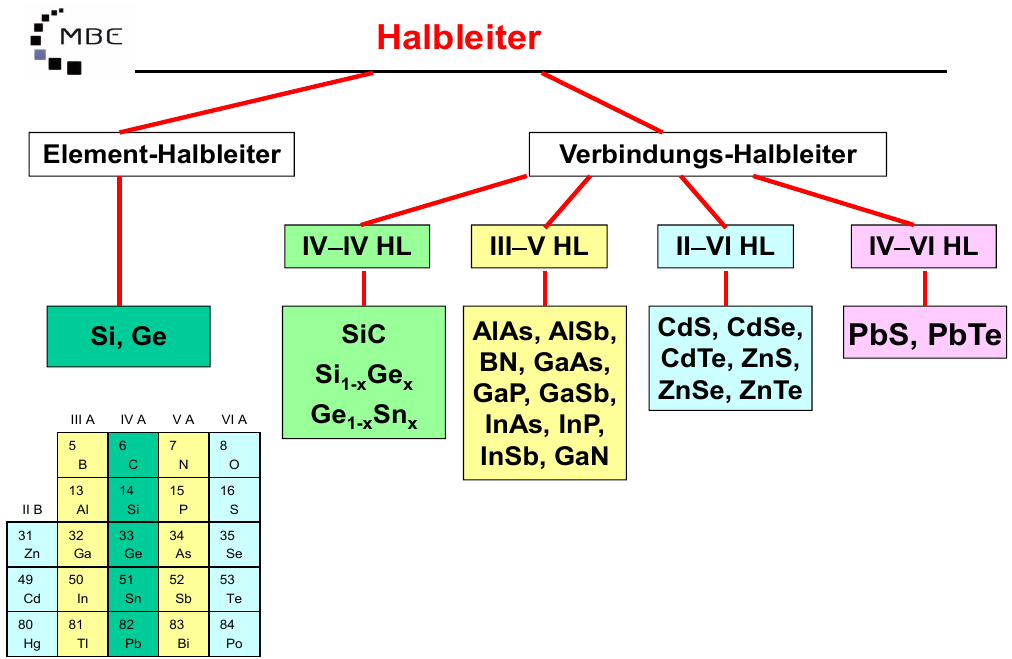
\includegraphics[width=0.8\textwidth]{Kapitel/Kap02/halbleiter.PNG}
		\caption{Halbleiter}
		\label{02_HL}
	\end{figure}
	\newpage
	
	
\subsection{Eigenschaften von Silizium}
	\subsubsection{Stellung im Periodensystem}
		Silizium befindet sich in der 4. Hauptgruppe und der 3. Periode im Periodensystem und hat die Ordnungszahl 14.
		\begin{figure}[h!]
			\centering
			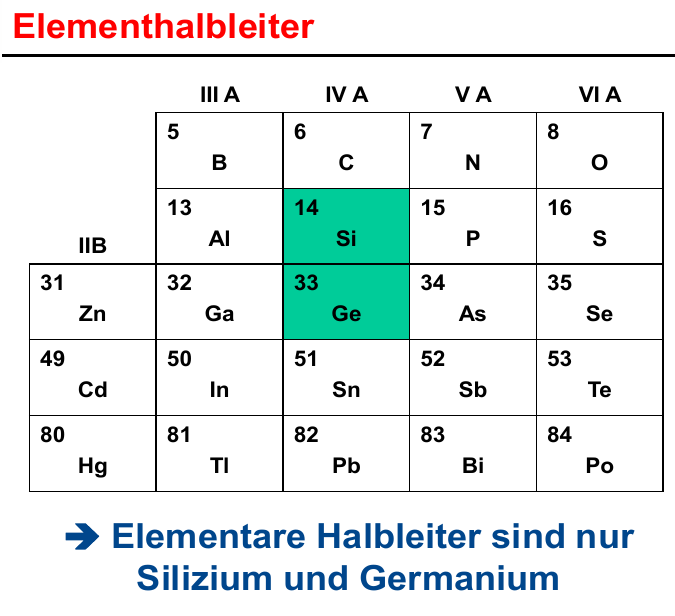
\includegraphics[width=0.5\textwidth]{Kapitel/Kap02/elementhalbleiter.PNG}
			\caption{Silizium im Periodensystem}
			\label{02_elementHL}
		\end{figure}
		
		
	\subsubsection{Valenzelektronen}
		Silizium ist ein indirekter Halbleiter. Damit ein ELektron aus dem Valenzband in das Leitungsband übergehen kann, muss ihm neben einer Energie auch noch ein Impuls zugeführt werden. Diese Art der Übergänge sind energetisch wenig wahrscheinlich.
		Die benötigte Energie ist hier die Energiedifferenz von Leitungsband zu Valenzband :
		\begin{equation*}
		E_g = E_{LB} - E_{VB}
		\end{equation*}
		
		Der benötigte Impuls beträgt:
		\begin{equation*}
			\Delta p = 2\pi h(k_{LB}-k_{VB})
		\end{equation*}
		
		Silizium hat eine Bandlücke von ca 1.1eV.
		
		\newpage
		\begin{figure}[ht]
			\centering
			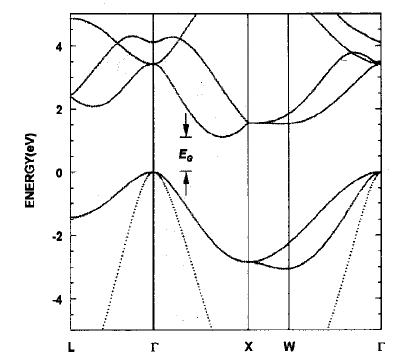
\includegraphics[width=0.5\textwidth]{Kapitel/Kap02/bandstruktur_SI.PNG}
			\caption{Bandstruktur von Silizium}
			\label{02_BS_SI}
		\end{figure}
		
	
	\subsubsection{Kristallstruktur}
		
		Kristallstruktur: Diamantstruktur
		Das Raumgitter besteht aus zwei kubisch-flächenzentrierten Gittern, die um 1/4 der Raumdiagonalen gegeneinander verschoben sind.
		Basis: identische Atome bei (0,0,0) und (1/4, 1/4, 1/4).
		Ein Si-Atom hat vier Außenelektronen, mit denen es Bindungen zu vier Nachbaratomen eingehen kann. Da (fast) alle Elektronen gebunden sind, ist die Leitfähigkeit (bei Raumtemperatur) sehr gering. (Das Valenzband ist (fast) vollständig besetzt, das Leitungsband hingegen (fast) vollständig leer.)
		
				
	\begin{figure}[h!]
		\centering
		\begin{minipage}[t]{0.35\linewidth}
			\centering
			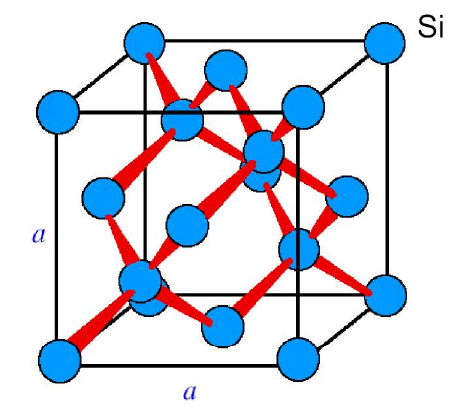
\includegraphics[width=\linewidth]{Kapitel/Kap02/Diamantstruktur_SI.PNG}
			\caption{Diamantstruktur von Silizium}
			\label{02_diamStruktur}
		\end{minipage}% <- sonst wird hier ein Leerzeichen eingefügt
		\hfill
		\begin{minipage}[t]{0.35\linewidth}
			\centering
			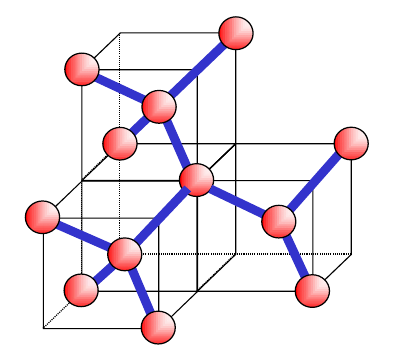
\includegraphics[width=\linewidth]{Kapitel/Kap02/raeumlichesModell_SI.PNG}
			\caption{räumliches Modell von Silizium}
			\label{02_raeumlModell}
		\end{minipage}
	\end{figure}

		
	\subsubsection{Miller'sche Indizes und Kristallorientierungen}
	
		In der heutigen Mikroelektronik wird überwiegend Si(001) genutzt.
		Die Oberfläche von Si(001) hat eine 4-fache Symmetrie, damit gibt es zwei freie Bindungen pro Oberflächenatom.
		Die Oberfläche von Si(111) hat dagegen eine 3-fache Symmetrie und damit nur eine freie Bindung pro Oberflächenatom.
		
		\begin{figure}[h]
			\centering
			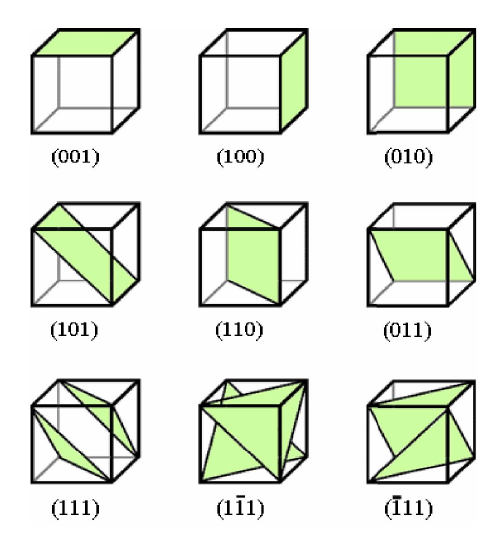
\includegraphics[width=0.22\textwidth]{Kapitel/Kap02/millerscheIndizes.PNG}
			\caption{Miller'sche Indizes}
			\label{02_millInd}
		\end{figure}
	
\subsection{Eigenleitung}
	T=0K: Alle möglichen Energiezustände im Valenzband sind von Elektronen besetzt. Das Leitungsband ist leer $\rightarrow$ es handelt sich um einen perfekten Isolator
	T>0K: Thermische Schwingungen können zur Bildung eines Elektron-Lochpaares führen. Die entstandenen freien Elektronen bedingen sich energetisch im Leitungsband. Die positiv geladenen Löcher verbleiben im Valenzband, sie sind dort ebenfalls beweglich.
	
	$Si \longrightarrow Si + e^- + h^+$ (e = electrons, h = holes)
	
	Im reinen Halbleiter finden Elektronenleitung \textbf{und} Löcherleitung statt. Die Anzahl von freien Elektronen und Löchern ist gleich: $\mathbf{n_i \cdot{p_i} = {n_i}^2}$
	
	\textbf{Generation:} Entstehung eines Elektron-Lochpaares
	\textbf{Rekombination:} Verschwinden eines Elektron-Lochpaares
	$\rightarrow$ hierbei fängt ein beliebiges Loch, unter Freigabe von Energie, ein beliebiges Elektron auf.
	
	Die Beweglichkeit von Elektronen ist immer sehr viel höher als die der Löcher.
	
\subsection{Dotierung}
	Die Eigenleitung von Halbleitern ist zu gering für eine technische Nutzung. Durch Dotierung (gezielte Verunreinigung mit Fremdatomen) wird die Leitfähigkeit erhöht. Die dotierten Materialien können überwiegend positive Ladungen (p-Typ) oder negative \textbf{freie} Ladungen (n-Typ) haben.
	Das \textbf{Massewirkungsgesetz} gilt aber auch für dotierte Halbleiter: $\mathbf{n \cdot{p} = {n_i}^2}$
	
	\subsubsection{Akzeptoren, Donatoren }
		\textbf{Donator:} ein Fremdatom der V-Hauptgruppe liefert ein zusätzliches Elektron
		Dotieren führt hier also zu einem Elektronenüberschuss $\rightarrow$ n-Leiter
		\begin{description}
			\item[$\bullet$] 5-wertige Stoffe sind z.B. Phosphor, Arsen, Antimon
			\item[$\bullet$] die abgegebenen Elektronen der Donatroren sind die (negativen) Ladungsträger
			\item[$\bullet$] es entstehen außerdem feste, positiv-geladene Ionen (tragen aber nicht zum Stromfluss bei)
			\item[$\bullet$] die Energieniveaus der Donatoren liegen dicht unterhalb des LB-Minimums in der Bandlücke ( $\rightarrow$ flache Störstelle)
		\end{description}
		
		\textbf{Akzeptor:} ein Fremdatom der III-Hauptgruppe kann ein Elektron aufnehmen
		Dotieren führt hier also zu einem Löcherüberschuss $\rightarrow$ p-Leiter
		\begin{description}
			\item[$\bullet$] 3-wertige Stoffe sind z.B. Bor, Gallium, ALuminium, Indium
			\item[$\bullet$] die entstehenden freien Löcher sind die (positiven) Ladungsträger
			\item[$\bullet$] es entstehen außerdem feste, negativ-geladene Ionen (tragen aber nicht zum Stromfluss bei)
			\item[$\bullet$] die Energieniveaus der Akzeptoren liegen dicht oberhalb des VB-Maximums in der Bandlücke ( $\rightarrow$ flache Störstelle)
		\end{description}
	
	\subsubsection{Konzentration, Lage im Bandgap usw.}
		
		
		\begin{figure}[h!]
			\centering
			\begin{minipage}[t]{0.45\linewidth}
				\centering
				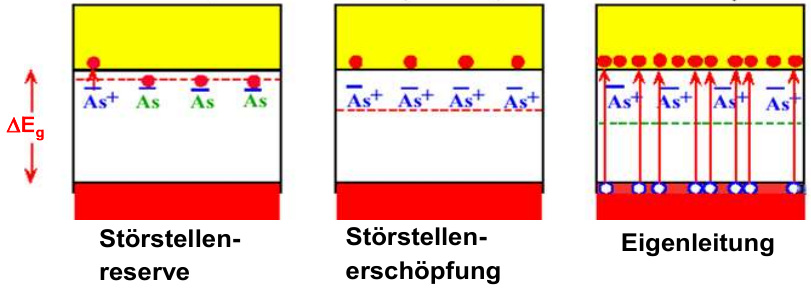
\includegraphics[width=1.2\textwidth]{Kapitel/Kap02/tempAbhSiAs.PNG}
				\caption{Dotieratomanregung am Beispiel von SiAs}
				\label{02_tempAbh}
			\end{minipage}% <- sonst wird hier ein Leerzeichen eingefügt
			\hfill
			\begin{minipage}[t]{0.45\linewidth}
				\centering
				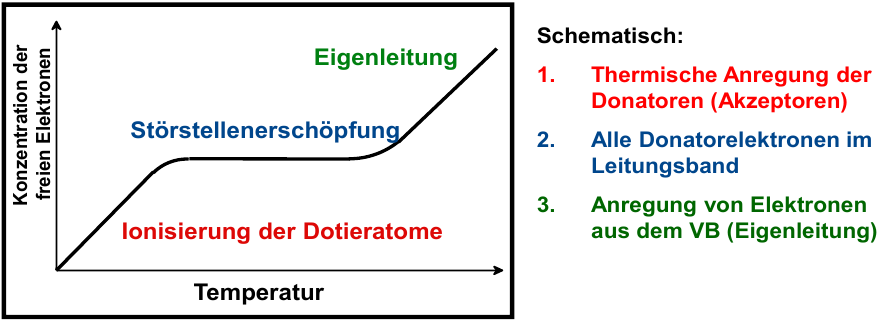
\includegraphics[width=1.2\textwidth]{Kapitel/Kap02/ladungstraegerkonzentration.PNG}
				\caption{T-Abhängigkeit der Ladungsträgerkonzentration (gilt auch für Akzeptoren)}
				\label{02_tempAbh2}
			\end{minipage}
		\end{figure}
		
		\begin{figure}[h!]
			\centering
			\begin{minipage}[t]{0.35\linewidth}
				\centering
				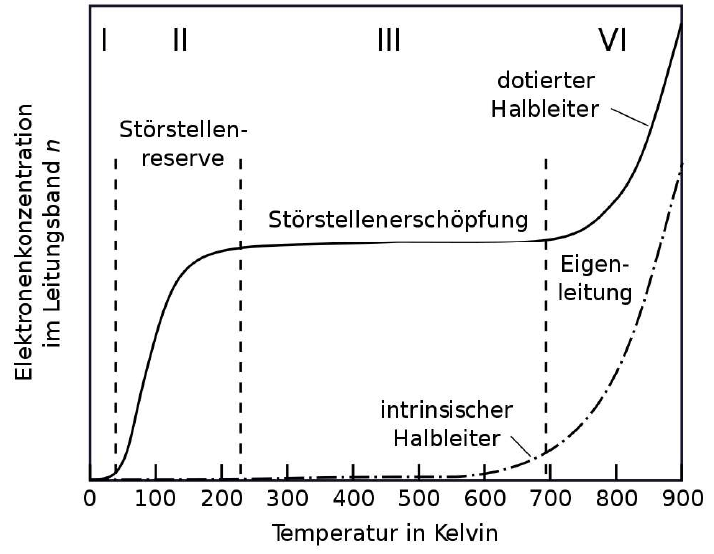
\includegraphics[width=\textwidth]{Kapitel/Kap02/tempAbh2.PNG}
				\caption{T-Abhängigkeit der Ladungsträgerkonzentration}
				\label{02_tempAbh3}
			\end{minipage}% <- sonst wird hier ein Leerzeichen eingefügt
			\hfill
			\begin{minipage}[t]{0.35\linewidth}
				\centering
				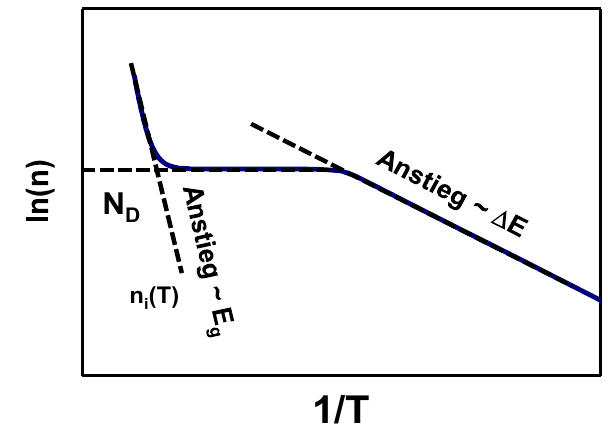
\includegraphics[width=\textwidth]{Kapitel/Kap02/tempAbh3.PNG}
				\caption{T-Abhängigkeit der Ladungsträgerkonzentration}
				\label{02_tempAbh4}
			\end{minipage}
		\end{figure}
		
		\newpage
		\textbf{Lage im Bandgap:}
		\begin{figure}[h!]
			\centering
			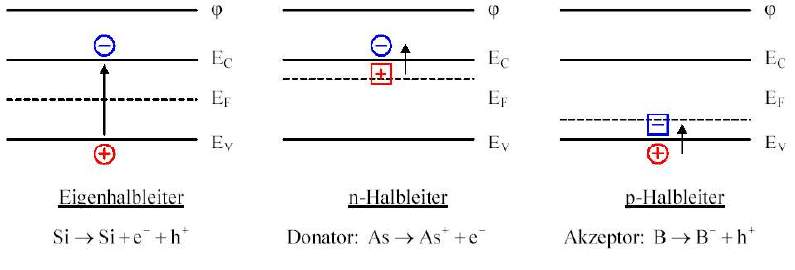
\includegraphics[width=0.9\textwidth]{Kapitel/Kap02/bandgapLage.PNG}
			\caption{Lage im Bandgap}
			\label{02_bandgap}
		\end{figure}
		
	\subsubsection{Dotantenaktivierung}
	DIe Anregung (Ionisation) wird als Aktivierung bezeichnet. Die Wahrscheinlichkeit für die Ionisation eines Donators ist von der Lage seines Energieniveaus $E_D$ abhängig. 
	Anzahl der Donatoren = neutrale + ionisierte ($N_D = {N_D}^0 + {N_D}^+$)
	\newpage
	
	\subsubsection{Dotiertechniken}
		\begin{figure}[h!]
			\centering
			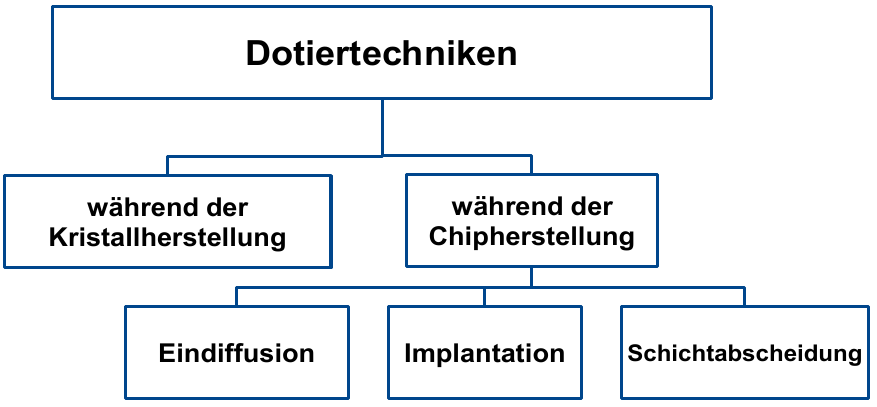
\includegraphics[width=0.7\textwidth]{Kapitel/Kap02/dotiertechniken.PNG}
			\label{02_dotiertechniken}
		\end{figure}
		
\subsection{Gewinnung von Reinstsilizium}

	\subsubsection{Reduktion im Niederschachtofen}
		Sand (Siliziumdioxid - $SiO_2$) wird bei ca 1450°C geschmolzen. Dabei wird Kohlenstoff zugegeben. Der Kohlenstoff verbindet sich mit dem Sauerstoff zu Kohlenmonoxid, was so aus der Schmelze entweicht. Die Reaktionsprodukte (Silizium und gasförmiges Kohlenmonoxid) lassen sich leicht trennen.
		\begin{figure}[h!]
			\centering
			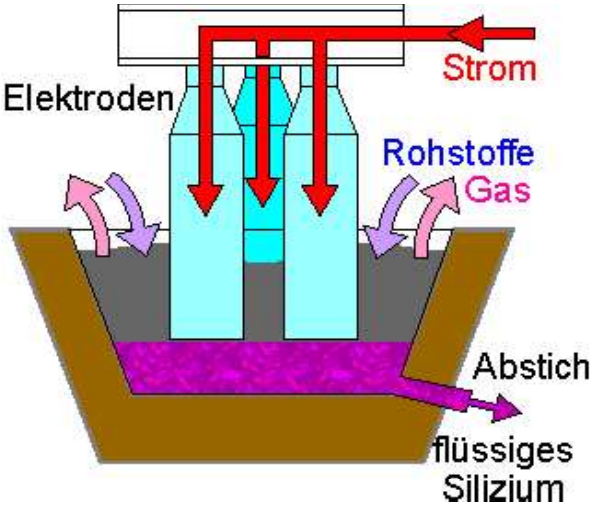
\includegraphics[width=0.4\textwidth]{Kapitel/Kap02/niederschachtofen.PNG}
			\caption{Niederschachtofen}
			\label{02_niederschachtofen}
		\end{figure}
		
	\subsubsection{Reinigung im Wirbelschichtreaktor}
		Das gewonnene Rohsilizium hat typischerweise immer noch Verunreinigungen von ca 2-4% , die entfernt werden müssen. Hierfür wird das Rohsilizium zu Trichlorsilan umgewandelt und anschließend fraktioniert destilliert. Um das Silizium umzuwandeln wird es zu einer Korngröße von ca 0.1mm gemahlen und dann in einem Wirbelschichtreaktor mit Chlorwasserstoff durchwirbelt. Unter Wärmeentwicklung entsteht als Reaktionsprodukt hauptsächlich Trichlorsilan.
		Trichlorsilan hat einen Siedepunkt von 30°C und kann deshalb in großen, mehrstufigen Destillationsanlagen von den Verunreinigungen befreit werden. Dieses gereinigte Trichlorsilan dient als Ausgangsstoff für die Herstellung von polykristalllinem Reinsilizium.
		
	\subsubsection{Polyabscheidung (Siemensprozess)}
		Trichlosilan und Wasserstoff werden in einen Abscheidungsreaktor geleitet. Dieser besteht aus einer Quarzglocke, in dem sich eine u-förmige Brücke aus dünnen Reinstsiliziumstäben (Dünnstab) befindet. Hier wird polykristallines Silizium abgeschieden. Durch den Dünnstab wird ein elektrischer Strom geleitet, der für die nötige Erwärmung auf die Reaktionstemperatur sorgt. (Je dicker der Stab wird, desto höher wird der Strom geregelt.) Das polykristalline Silizium hat nun eine Reinheit von 99,9999999% (9N).
\subsection{Einkristallines Silizium}
	Für die Chipherstellung wird einkristallines Silizium benötigt. Der Einkristall wird aus dem polykristallinen Silizium gezogen. Hierfür gibt es zwei Verfahren: Zonenziehen und Tiegelziehen im Schmelztiegel. Bei beiden Verfahren wird ein Impfkristall verwendet. Dies ist ein kleiner Einkristall mit einer genau definierten Ausrichtung des Kristallgitters. Die Kristallstruktur des erstarrenden Siliziums richtet sich genau an der des Impfkristalls aus $\Rightarrow$ Epitaxie
	
	\subsubsection{Zonenziehen und Tiegelziehen}
		\textcolor{red}{\textbf{Zonenziehen:}} (FZ-Verfahren)
			Silizium in Stabform wird mit einer Hochfrequenz-Induktionsspule direkt beheizt. Nach dem Anschmelzen wird der Schmelztropfen mit dem Impfkristall in Kontakt gebracht. Der sich drehende Stab wird durch die Spule abgesenkt und die Schmelzzone somit von unten nach oben gezogen.
			
			\textbf{Vorteile:}
				\begin{description}
					\item[$\bullet$] noch bestehenden Verunreinigungen werden in der Schmelze gelöst und so aus dem Stab herausgezogen
					\item[$\bullet$] Dotierungen, in Form von Prozessgasen, können gezielt vorgenommen und homogen in das Kristallgitter eingebaut werden
				\end{description}
			\textbf{Nachteile:}
			\begin{description}
				\item[$\bullet$] es lassen sich nur Stäbe von einem Durchmesser von 150mm sinnvoll ziehen
			\end{description}
				
			
		\textcolor{red}{\textbf{Tiegelziehen:}} (CZ-Verfahren)
		
		\begin{figure}[h!]
			\centering
			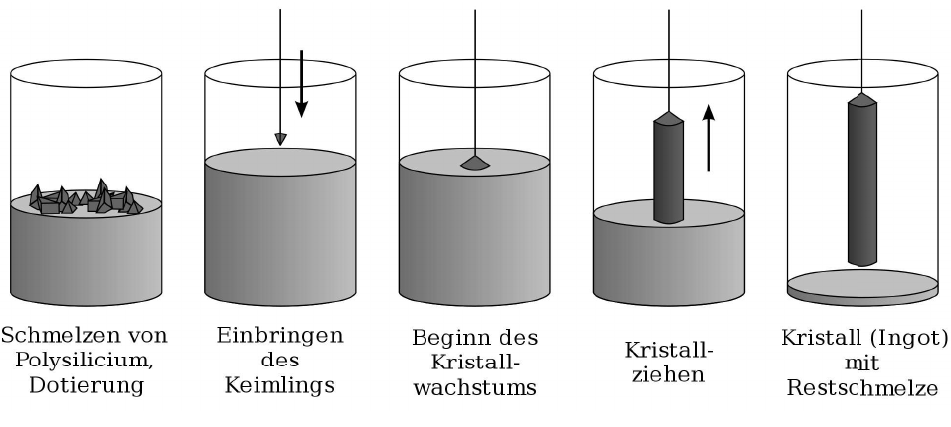
\includegraphics[width=\textwidth]{Kapitel/Kap02/tiegelziehen.PNG}
			\caption{Tiegelziehen}
			\label{02_tiegelziehen}
		\end{figure}
		
		\textbf{Vorteile:}
		\begin{description}
			\item[$\bullet$] ist vorallem für die Produktion von modernen großen Wafern geeignet (300mm und größer)
		\end{description}
		\textbf{Nachteile:}
		\begin{description}
			\item[$\bullet$] Dauer des Ziehprozesses: 1-3 Tage
			\item[$\bullet$] Inhomogenität bei der Vordotierung
			\item[$\bullet$] Verunreinigungen entstehen durch Kohlenstoff und Sauerstoff im Tiegel (die Verunreinigungen sind für viele Anwendungen aber gering genug)
		\end{description}
		
	\subsubsection{Zusammenfassung: Gewinnung von einkristallinem Silizium}
		\begin{description}
			\item[$\bullet$] \textbf{Gewinnung von Rohsilizium}
			\begin{description}
				\item[-] Reduktion im Niederschachtofen
				\item[-] Reinigung im Wirbelschichtreaktor $\rightarrow$ Umwandlung in Trichlorsilan
				\item[-] Polyabscheiung (Siemensprozess) $\rightarrow$ polykristallines Reinsilizium
			\end{description}
			\item[$\bullet$]Einkristallines Silizium
			\begin{description}
				\item[-] Zonenziehen oder Tiegelziehen
			\end{description}
			$\Rightarrow$ Einkristalline Si-Blöcke
		\end{description}
		
	\subsubsection{Wafermaße und -orientierungen}
		\begin{figure}[h!]
			\centering
			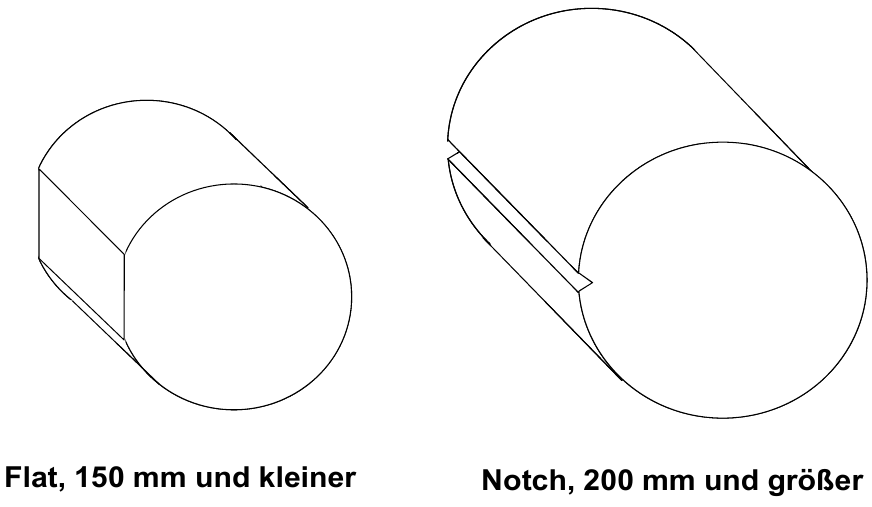
\includegraphics[width=0.4\textwidth]{Kapitel/Kap02/wafermasse.PNG}
			\caption{Flat oder Notch}
			\label{02_flat_notch}
		\end{figure}
		
		\begin{figure}[h!]
			\centering
			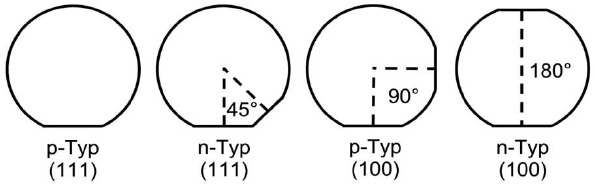
\includegraphics[width=0.6\textwidth]{Kapitel/Kap02/orientierungen.PNG}
			\caption{Waferherstellung: Flat}
			\label{02_flat}
		\end{figure}

	\todo{Fragen aus Own Clowd zuordnen}
	\todo{Gruppenübungs-Inhalte ergänze}

	
	% Kapitel 3
	\section{Kapitel 3 - Bandstruktur }
	\todo{Wichtige Begriffe erklären}
\subsection{Interferenz}
	\subsubsection{Verstärkung, Auslöschung, Weg- bzw. Phasenunterschied}
\subsection{Elektronen als Welle}
	\subsubsection{De Broglie Beziehung, Impuls, Wellenzahl usw.}
\subsection{Überlagerung von zwei Wellen}
	\subsubsection{Gleiche Wellen, entgegenlaufende Wellen, stehende Welle}
\subsection{Elektronen im Kastenpotential}
	\subsubsection{Einfacher Kasten, periodisches Kristallgitter}
\subsection{Bandstruktur von Halbleitern}
	\textbf{Bändermodell allgemein:}
	\begin{description}
		\item[Leitungsband:] Freie Elektronen (nicht mehr an ein bestimmtes Atom gebunden = Stromleitung möglich)
		\item[Bandlücke:] 'Verbotene Zone' $\rightarrow$ Energiebereich, ohne erlaubte Energieniveaus für Elektronen
		\item[Valenzband:] Energiebereich, in dem sich die äußeren Bindungselektronen des Atoms befinden (nicht für Stromleitung verfügbar) 
	\end{description}
	
	
	\subsubsection{Bandlücke, Brillouin-Zone
	Temperaturabhängigkeit}

		\textbf{Bandlücke bei Festkörpern:}
		\begin{description}
			\item[Metalle:] keine Bandlücke ($E_g$ = 0)
			\item[Isolatoren:] $E_g$ > 3eV
			\item[Halbleiter:] $E_g$ < 3eV
		\end{description}
		
		
\subsection{Direkte und indirekte Halbleiter}
	\begin{figure}[h!]
		\centering
		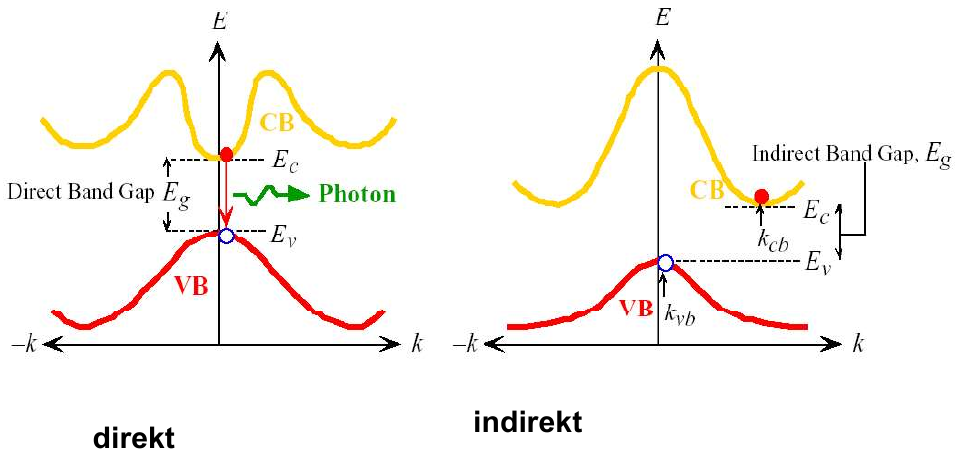
\includegraphics[width=\textwidth]{Kapitel/Kap03/uebergang_direkt_indirekt.png}
		\caption{direkter vs. indirekter Übergang}
		\label{02_uebergang}
	\end{figure}
	
	Für den Übergang von einem Elektron aus dem Valenzband ins Leitungsband ist bei einem direkten Halbleiter keine Impulsänderung notwendig; bei einem indirekten Halbleiter hingegen schon.
	
	\begin{figure}[h!]
		\centering
		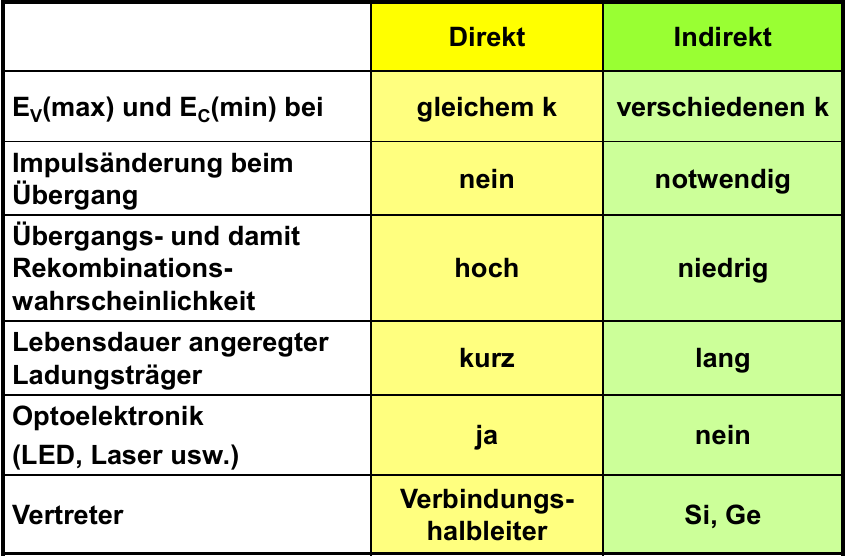
\includegraphics[width=0.8\textwidth]{Kapitel/Kap03/direkt_indirekt.png}
		\caption{direkter vs. indirekter Halbleiter}
		\label{02_dir_ind_hl}
	\end{figure}
	
\subsection{Effektive Massen}
	Es kann an den Minima und Maxima im Bändermodell unertschiedliche $E(k)$ -Funktionen geben, dies nennt man entartet. 
	Je flacher das Leitungsband am Minimum ist, desto schwerer wird die effektive Masse der Elektronen. Es gibt also 'schwere' und 'leichte' Massen (z.B. hh : heavy holes und lh: light holes), es können demnach auch heavy holes und light holes zusammen an den Maxima und Minima auftreten.
	Alle Massen tragen gewichtet nach ihren Anteilen zum Ladungstransport bei. 
	$\rightarrow$ analoges gilt auch für Löcher
	
	\begin{figure}[h!]
		\centering
		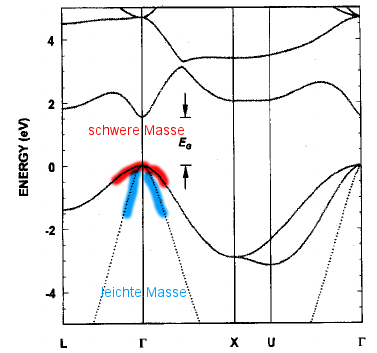
\includegraphics[width=0.3\textwidth]{Kapitel/Kap03/effektiveMasse.png}
		\caption{Beispiel: GaAs}
		\label{02_effMasse}
	\end{figure}

	Die Geschwindigkeit der Ladungsträger ist proportional zur elektrischen Feldstärke:
	\begin{equation*}
		v_n = {-\mu}_n E \quad \textrm{ und } \quad v_p = {\mu}_p E
	\end{equation*}
	
	Die Proportionalitätskonstante wird als \textbf{Beweglichkeit} bezeichnet. Wobei die Beweglichkeit mit steigender Masse abnimmt: ${\mu} \sim \frac{1}{m^*}$ ($m^* = effektive Masse$)
	Die Beweglichkeit von Löchern und Elektronen ist unterschiedlich.
	
\subsection{Verspanntes Silizium}
	Verpsannt man Silizium, so hebt man die Entartung auf. Die Ladungsträger werden so energetisch günstiger für den Transport.
	\begin{figure}[h!]
		\centering
		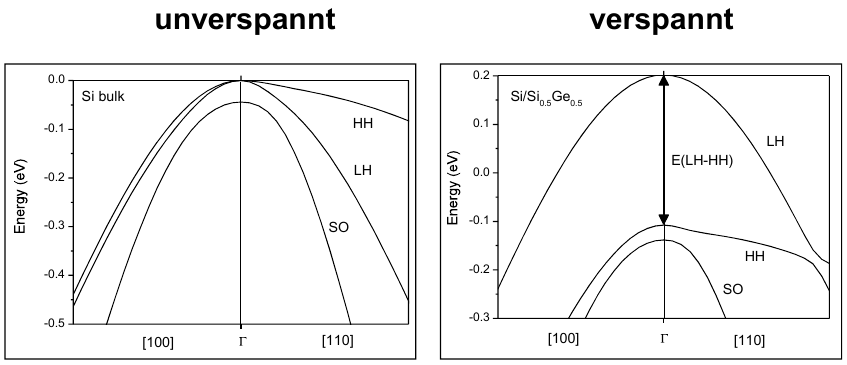
\includegraphics[width=0.5\textwidth]{Kapitel/Kap03/verspanntesSi.png}
		\caption{Spannungseinfluss im Valenzband (Silizium)}
		\label{02_verspSi}
	\end{figure}
	
\todo{Fragen aus Own Clowd zuordnen}
\todo{Gruppenübungs-Inhalte ergänzen}
	
	% Kapitel 4
	\section{Kapitel 4 - Ladungsträger }
	\todo{Wichtige Begriffe erklären}
\subsection{Verteilungsfunktion}
	\subsubsection{Fermiverteilung}
	\subsubsection{Definition der Fermi-Energie}	
	\subsubsection{Lage des Fermi-Niveaus (intrinsisch vs. dotiert)}
	\subsubsection{Effektive Zustandsdichten}	
\subsection{Ladungsträger im Halbleiter}
	\subsubsection{Massenwirkungsgesetz}
	\subsubsection{Neutralitätsbedingung}
	\subsubsection{Intrinsische Ladungsträgerkonzentration}
	\subsubsection{Bezeichnung von dotierten Halbleitern}
	\subsubsection{Majoritäten und Minoritäten}
\subsection{Ladungsträgerbewegung}
	\subsubsection{Driftstrom, Sättigung usw.}
	\subsubsection{Diffusionsstrom}
	\subsubsection{Temperaturspannung}	
\subsection{Leitfähigkeit von Halbleitern}
	\subsubsection{p- und n-Typ, Temperaturabhängigkeit usw.}
	\subsubsection{Definitionen von Dotierniveaus}



\todo{Fragen aus Own Clowd zuordnen}
\todo{Gruppenübungs-Inhalte ergänzen}
	
	% Kapitel 5
	\section{Kapitel 5 - Ladungsträgerdynamik }
	\subsection{Fermi-Verteilung}
Fermi-Verteilung ist Ergebnis eines dynamischen Gleichgewichts bei einer Temperatur
\subsection{Fermi-Niveau im Nichtgleichgewicht}
	
	\subsection{Generation und Rekombination}
		Generation ist Erzeugung von Ladungsträgern (eines Elektrons und eines Lochs) unter Energiezufuhr (Wärme, Strahlung usw.).
		\newline
		
		Rekombination ist der Übergangsprozess von einem Elektron aus dem Leitungsband-Zustand in einen Valenzband-Zustand. Unter Energieabgabe werden so Ladungsträger
		(Elektronen und Löcher) vernichtet.
		\newline
		
		Bei diesen Prozessen bleibt die Gesamtladung erhalten.
		\newline
		
		Im thermischen Gleichgewicht sind G und R gleich groß
		\newline
		
	\subsubsection{Überschuss-Ladungsträger}
	
	Überschuss-Ladungsträger ergibt sich aus dem Delta der Anzahl der freien Elektronen n und der Freien Elektronen bei Eigenleitung $n_0$
	\newline
	$\Delta n=n - n_0$
	
	\subsection{Lebensdauer}
	Ladungsträgerlebensdauer ergibt sich aus dem Quotient aus Überschuss-Ladungsträgern $\Delta n$ und Rekombinationsrate R
	\newline
	
	$\tau =\frac{\Delta n}{R}$
	
	
	\subsubsection{Rekombinationsrate}

	Die Rekombinationsrate R ist der Quotient aus Überschussladungsträgern und der Ladungsträgerlebensdauer $\tau$
 
		$R =\frac{\Delta n}{\tau}$
		\newline
		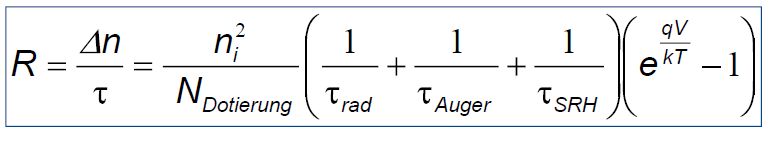
\includegraphics[width=0.4\linewidth]{Kapitel/Kap05/Rekombinationsrate}
		

	
	\subsubsection{Verschiedene Rekombinationsmechanismen}
	Es gibt verschiedene Rekombinationsmechanismen.
	\begin{enumerate}
		\item Strahlende Rekombination:
			\newline
			Elektron springt durch Energieabgabe durch Aussenden von Licht vom Leitungsband ins Valenzband. (Funtermentaler Prozess der direkten Halbleiter)
		\item Auger-Rekombination:
			\newline
			Auger-Rekombination ist ein sog. strahlungsloser Übergang. Sie benötigt drei Ladungsträger. Dabei wird die Energiedifferenz, die ein Elektron vom Sprung von Leitungs- in das Valenzband abgibt auf ein anderes Elektron übertragen, welches auf ein höheres Energieniveau gehoben wird. 
			\newline
			Mit zunehmender Ladungsträgerkonzentration (z.B. bei starker Dotierung) erhöht sich die Rekombinationsrate
		\item Defekt-Rekombination (Shockley-Read-Hall):
			\newline
			Die Defekt-Rekombination ist ein zwei-Stufen-Prozess, bei dem ein Elektron über einen Defektzustand/Störstelle (z.B. eine Verunreinigung durch andere Metalle) vom Leitungsband in das Valenzband spring. Die Energiedifferenz wird durch Aussendung von Licht bewirkt.
			\newline
			Es handelt sich um den Hauptverlustmechanismus in Silizium-basierten Bauelementen (Verringerung von Ladunsträgerlebensdauer). Die (geringe) Defektdichte (z.B. Verunreinigung, Kristallfehlordnung) ist daher das Maß für die Materialqualität.
		\item Oberflächen-Rekombination:
			\newline
			An Oberflächen des Halbleiters existieren lokalisierte Zustände,
			die sich nicht in die Bandstruktur einfügen. Die Rekombination findet wie bei der SRH statt.
			Oberflächenrekombination kann nur in Kombination mit Ladungsträgertransport zur Oberfläche geschehen.
			Rekombination am Metallkontakt läuft über die kontinuierliche
			Zustandsverteilung des Metalles ab und wird nür über den Transport der Ladungsträger im Halbleiter limitiert.
	\end{enumerate}



\begin{center}
	
	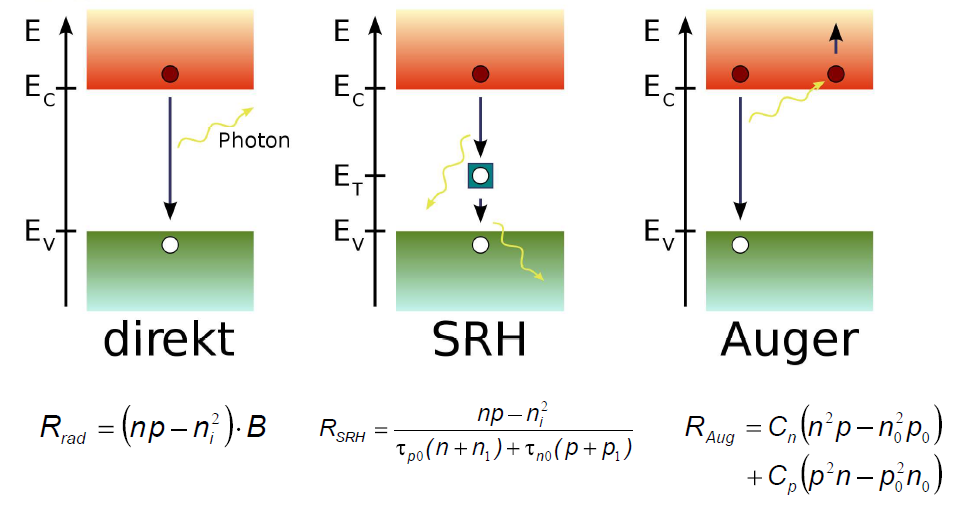
\includegraphics[width=0.7\linewidth]{Kapitel/Kap05/Rekombinationsarten1.png}
	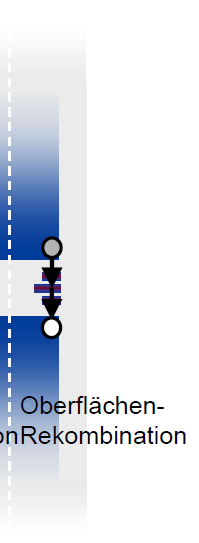
\includegraphics[width=0.15\linewidth]{Kapitel/Kap05/Rekombinationsarten2}
\end{center}

	
\subsection{Ortsabhängiges Energiebanddiagramm}
	Betrachtet man Halbleiter so ist zu Erkennen, dass die Energiebänder verbogen und damit Ortsabhängig sind.

\begin{center}
	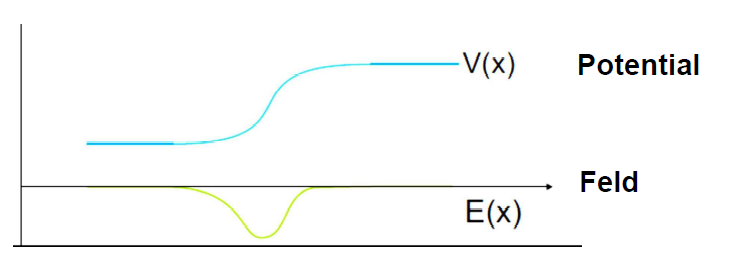
\includegraphics[width=0.5\linewidth]{Kapitel/Kap05/Ortsabhaengiges_Energiebanddiagramm.png}
	$E(x) = \frac{\delta V(x)}{\delta x}$
\end{center}





\subsection{Poisson-Gleichung}
Mit Hilfe der Poisson-Gleichung ist es möglich, die Bandverbiegung mit den Ladungsverteilungen im Inneren des HL in Verbindung zu bringen.

\begin{center}
	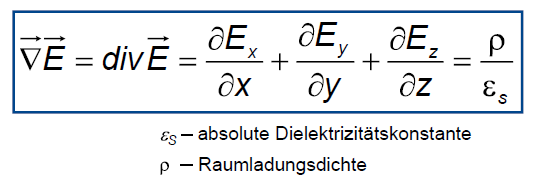
\includegraphics[width=0.5\linewidth]{Kapitel/Kap05/Poissongleichung}
\end{center}
Die hier als Poisson-Gleichung bezeichnete Maxwell'sche Gleichung, stellt einen allgemein gültigen Zusammenhang zwischen der Raumladungsdichte und dem Elektrischen Feld dar.

\subsubsection{Gradienten und Ströme}
Wenn Fermi-Level als "Füllstand" angesehen werden kann, dann erzeugt ein Gradient des Füllstandes einen Strom:

\begin{center}
	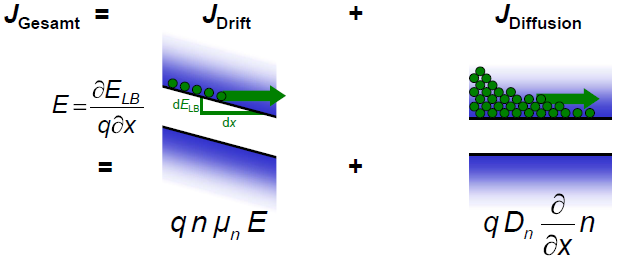
\includegraphics[width=0.7\linewidth]{Kapitel/Kap05/Gradient}
\end{center}
Gradient des Fermi-Levels gibt Netto-Stromrichtung an
\begin{center}
	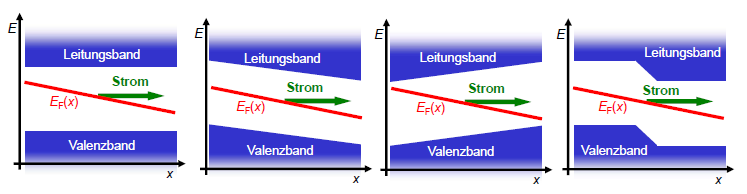
\includegraphics[width=0.6\linewidth]{Kapitel/Kap05/FerminiveauverlaufBeispiele}
\end{center}
Wenn der Verlauf des Fermi-Levels bekannt ist, d.h. der Gradient des Fermilevels, so ist die Richtung des Stromes gegeben, unabhängig von Bandkanten- (Feld-) Verlauf!

\subsection{Kontinuitätsgleichung}
Die Kontinuitätsgleichung vereint  Transport-, Rekombinations- und Generationsmechanismen in einer Gleichung, auf Basis der Ladungsträgererhaltung

\begin{center}
	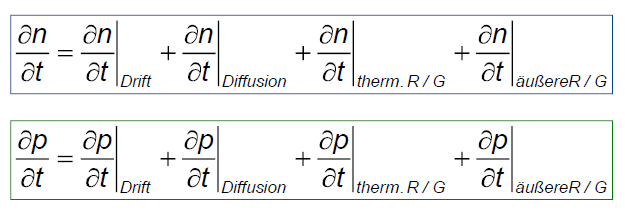
\includegraphics[width=0.7\linewidth]{Kapitel/Kap05/Kontinuitaetsgleichung}
\end{center}

Der Gesamtstrom hängt linear ab von:
\begin{itemize}
	\item der Beweglichkeit der Ladungsträger
	\item der Feldstärke (angelegten Spannung)
	\item dem Gradienten der Ladungsträgerkonzentration
\end{itemize}

\subsection{Minoritätsladungsträger-Diffusion}
	Zu viele Details --> vermutlich nicht relevant
	
	\subsubsection{Lösungen für Spezialfälle}
	Zu viele Details --> vermutlich nicht relevant
	
	
\subsection{Zwei Halbleiter im Kontakt}
	Kommen zwei Halbleiter in Kontakt hat man einen Halbleiterübergang, der aus verschiedenen oder verschieden dotierten Materialien besteht.
	Hierbei unterscheidet man zwischen:

	\begin{itemize}
		\item Homoübergang: Beide Halbleiter bestehen aus demselben Material 
		\item Heteroübergang: Beide Halbleiter bestehen aus verschiedenen Materialien und haben verschiedene Bandlücken		
	\end{itemize}
	Die Dotierung der beiden Materialen kann vom gleichen Typ oder entgegengesetzt sein (pn-Übergang)
	\subsubsection{Offsets, Typ I, II, III}
	Der Offset beschreibt den Übergang der Bandlücke (das Delta) zwischen den Leitungs- bzw. Valenzbändern der beiden Materialien. Bandoffsets können Barrieren sein.
	
	% offset graphik
	\begin{center}			
		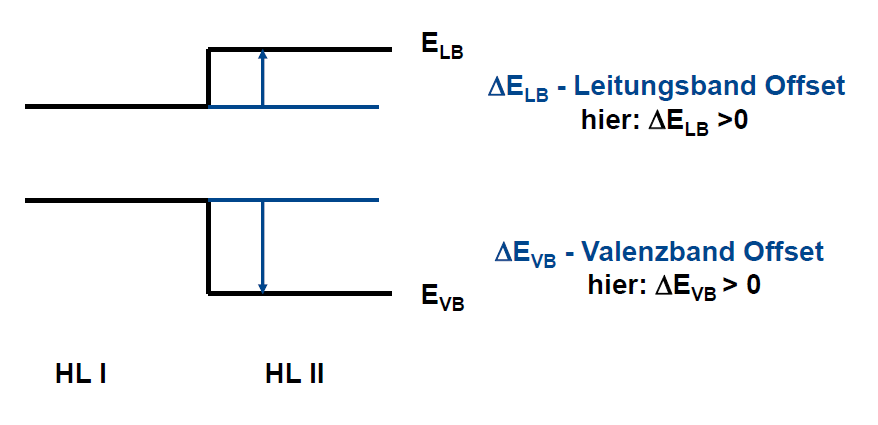
\includegraphics[width=0.7\linewidth]{Kapitel/Kap05/Offset.png}
	\end{center}
	
	Auf Basis des Offsets unterscheidet man zwischen drei Typen von Heteromaterialien:
	
	\begin{center}
	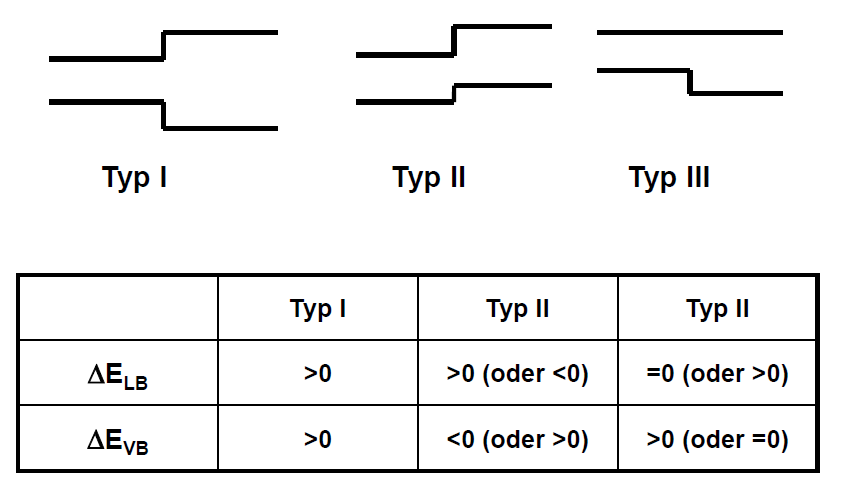
\includegraphics[width=0.7\linewidth]{Kapitel/Kap05/TypI-III}
	\end{center}
	
	\subsubsection{Injektion, Akkumulation, Extraktion, Exklusion}
	(Dieses Block wurde nicht in der Klausurenzusammenfassung der Übung erwähnt, der Vollständigkeitshalber wurde er mit aufgenommen)
	\newline
	Sind zwei Halbleiter in Kontakt gibt es unterschiedliche Beweglichkeiten und unterschiedliche Diffusion in beiden HLn.
	
	Hierbei gibt es Verschiedene Diffusions- und Driftströme
	Hierbei unterscheidet man 4 Arten
	\newline
		\begin{center}
			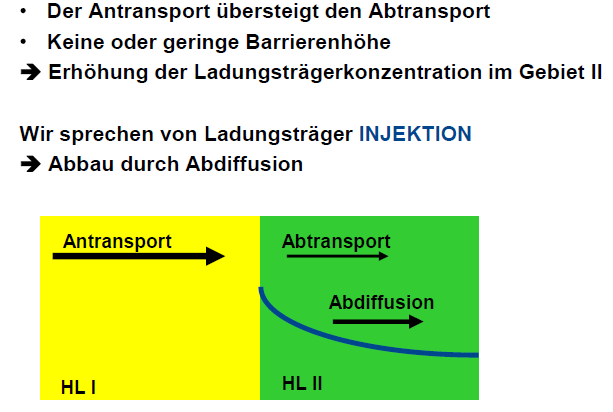
\includegraphics[width=0.45\linewidth]{Kapitel/Kap05/Interjektion}
			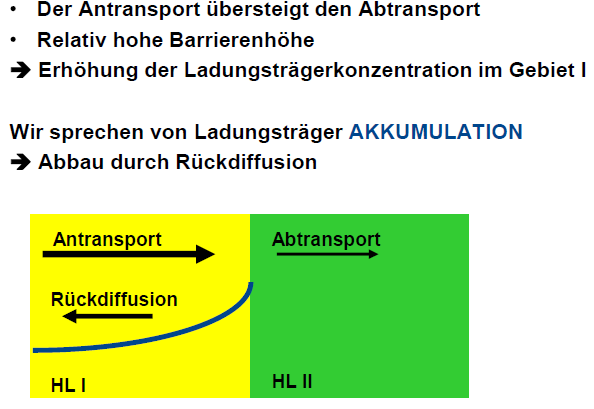
\includegraphics[width=0.45\linewidth]{Kapitel/Kap05/Akkumulation}
		\end{center}
	
		\begin{center}
			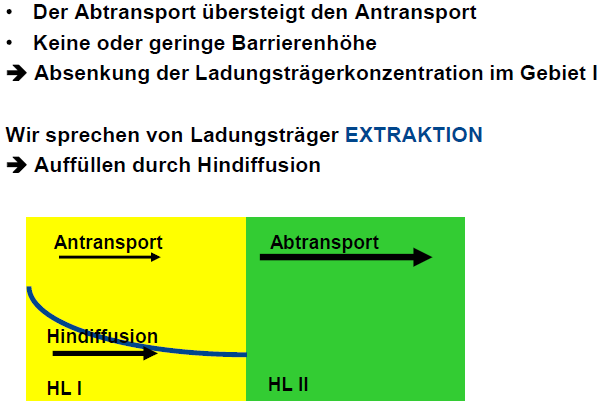
\includegraphics[width=0.45\linewidth]{Kapitel/Kap05/Extraktion}
			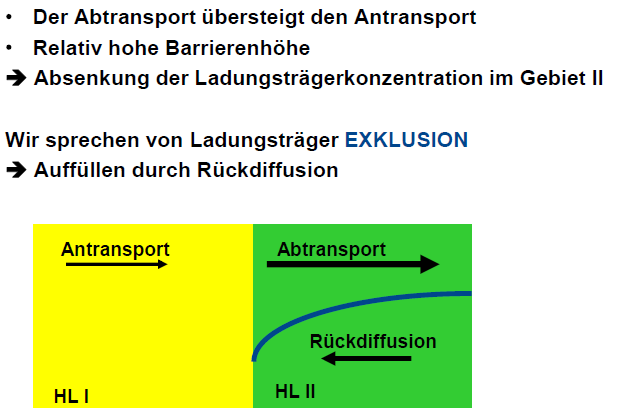
\includegraphics[width=0.45\linewidth]{Kapitel/Kap05/Exlusion}		
		\end{center}
			
\todo{Fragen aus Own Clowd zuordnen}
\todo{Gruppenübungs-Inhalte ergänzen}
	
	% Kapitel 6
	\section{Kapitel 6 - Feldeffekttransistor }
	\subsection{Was bedeutet MOS-Technologie}
MOS steht für Metal Oxide Semiconductor.
Sie heißen auch unipolar: nur ein Ladungsträgertyp ist am Stromtransport beteiligt
	\subsubsection{NMOS/PMOS}
		NMOS bzw. PMOS sind nach der im Kanal entstehenden n- bzw. p-Leitung benannt.
	\subsubsection{CMOS}
		CMOS steht für Complementary MOS.
		Hierbei handelt es sich um eine kombinierte Verwendung von NMOS- und PMOS-Transistoren in einem Schaltkreis. Diese Anordnung ist stromsparend, hat eine geringe Verlustleistung und hoher Integrationsgrad.
\subsection{MOS-Kondensatoren}
	Die allgemeinere Bezeichung ist MIS-Kondensator. MIS - metal insulator semiconductor. Wobei der der Isolator  häufig aus Siliziumdioxid besteht
	\subsubsection{Grundaufbau}
	Der MOS-Kondensator besteht aus 
	\begin{itemize}
		\item Metallelektrode
		\item Isolator
		\item dotiertem Silizium		
	\end{itemize}	
	\begin{center}
		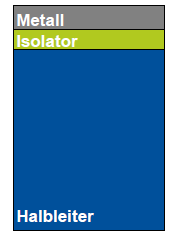
\includegraphics[width=0.2\linewidth]{Kapitel/Kap06/MOSKondensator}
	\end{center}
	
	\subsubsection{Flachbandfall}
		Background: im thermischen Gleichgewicht kommt es zu einem Ausgleich der unterschiedlichen Fermi-Niveaus (Halbleiter und Metall)
		\begin{itemize}
			\item Spannungsunterschied wird als Kontaktpotenzial bezeichnet
			\item 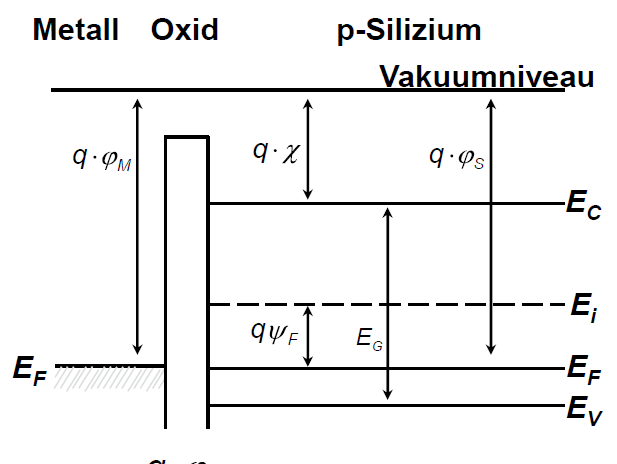
\includegraphics[width=0.4\linewidth]{Kapitel/Kap06/Kontaktpotential} 			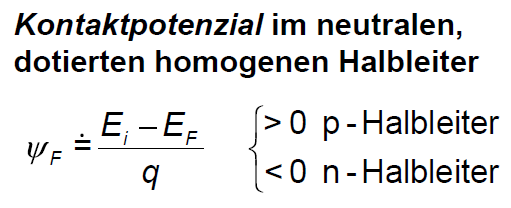
\includegraphics[width=0.4\linewidth]{Kapitel/Kap06/Kontaktpotential2}
			
			\item es bilden sich an der Grenzschicht zwischen Metall und Isolator positive und dem entgegengesetzt an der Grenzschicht zwischen Isolator und Halbleiter negative Ladungen aus.
			\item Es bildet sich eine Raumladungszone im Halbleiter			 		
		\end{itemize}
		Wichtig: Gleicht man das Kontaktpotenzial und den Spannungsabfall über das Oxid durch eine bestimmte schwache 	Vorspannung aus, so verschwindet die Raumladungszone man spricht vom Flachbandfall und der angelegten Flachbandspannung $U_{FB}$.
		
	\newpage
		
	\subsubsection{Anreicherung/Akkumulation, Verarmung, Inversion}
		Arbeitszustände (in diesen Fällen für für p-Silizium Substrate):
		\newline
		!!! Diagramme dienen nur der Veranschaulichung, Inversionsdiagramme sind wichtig !!!!
		\newline
		\textbf{Akkumulation:}
		\newline
		Beim Anlegen einer negative Spannung ($U_{MS} < 0 V $) gegenüber dem Substrat wandern die positiven Ladungsträger im Substrat zur 		Grenzschicht, sammeln sich dort und bilden eine Anreicherungszone
		\newline
		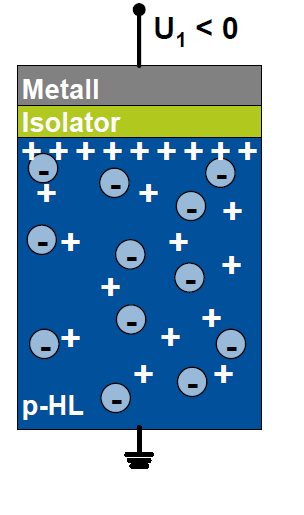
\includegraphics[width=0.25\linewidth]{Kapitel/Kap06/Akkumulation1}		
		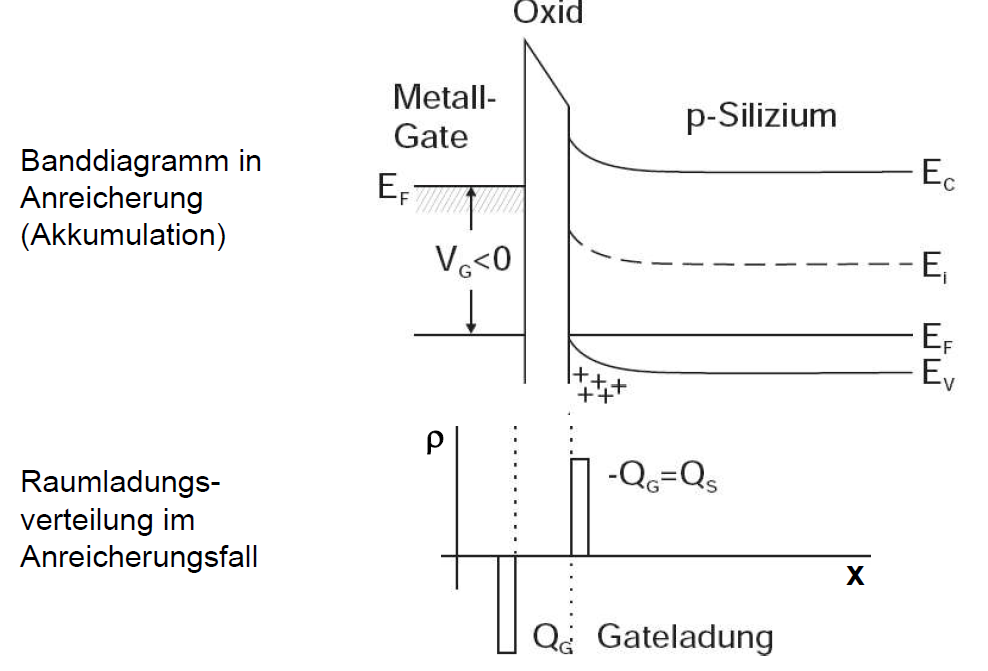
\includegraphics[width=0.60\linewidth]{Kapitel/Kap06/Akkumulation}
		\newline
		\newline
		
		\textbf{Verarmung:}
		\newline
		Bei Anlegen des Pluspols am Metall und
		des negativen Pols am Substrat ($U_{MS} > 0V$) wandern negative Ladungs-träger
		(Minoritäten) im Substrat an die Grenzschicht und rekombinieren mit den dort befindlichen freien positiven Ladungsträgern.
		\newline 
		In der Nähe der Grenzschicht entsteht durch die Rekombinationen eine 		Raumladungszone, die an freien 		Ladungsträgern verarmt ist. Diese Zone wird als Verarmungszone bezeichnet.
		\newline
		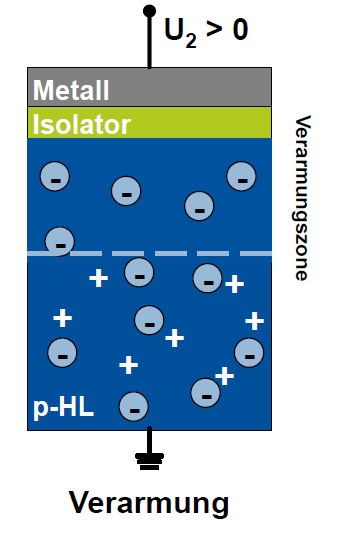
\includegraphics[width=0.25\linewidth]{Kapitel/Kap06/Verarmungszone1}
		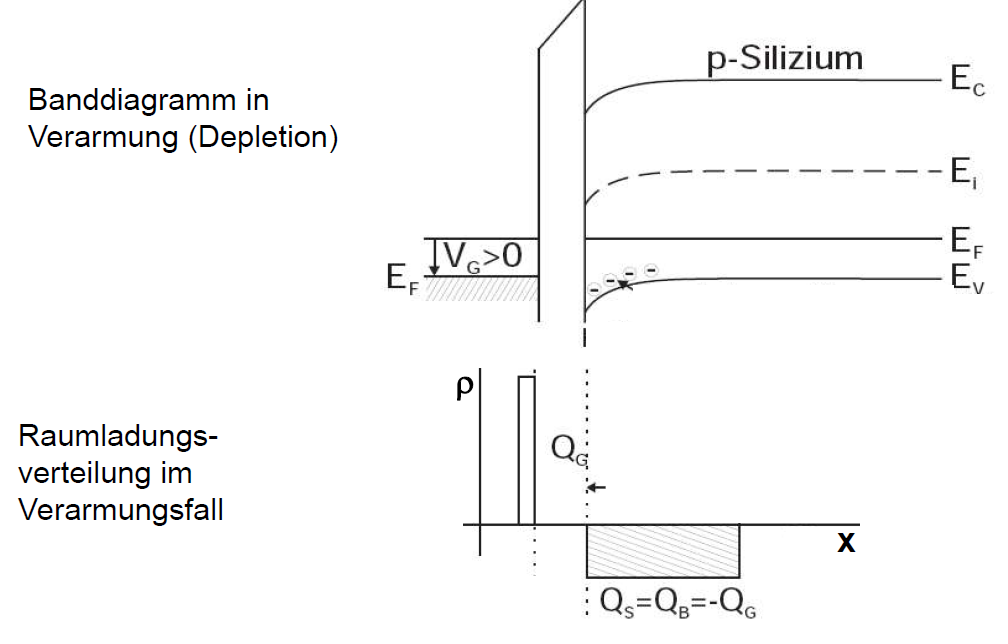
\includegraphics[width=0.60\linewidth]{Kapitel/Kap06/Verarmungszone2}
		
		\textbf{Inverstion:}
		\newline
		Überschreitet die angelegte Spannung eine Schwellspannung ($U_{MS} > U_{th}$ ,Threshold) bildet sich im ursprünglich p-dotierten Substrat ein n-dotiertes Gebiet. Es stehen keine freien Löcher mehr an der Grenzschicht zur Rekombination zur Verfügung.
		\newline
		Die so entstandene Zone, die die frei beweglichen negativen Ladungsträger enthält, wird als Inversionszone 	bezeichnet.
		\newline
		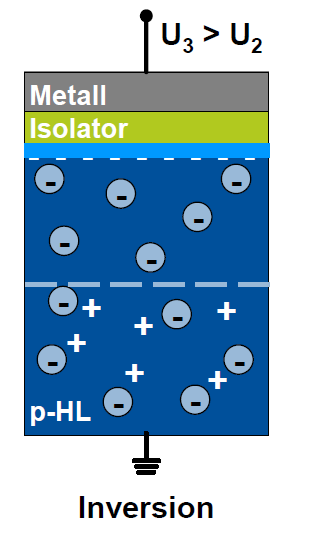
\includegraphics[width=0.25\linewidth]{Kapitel/Kap06/Inverstion1}		
		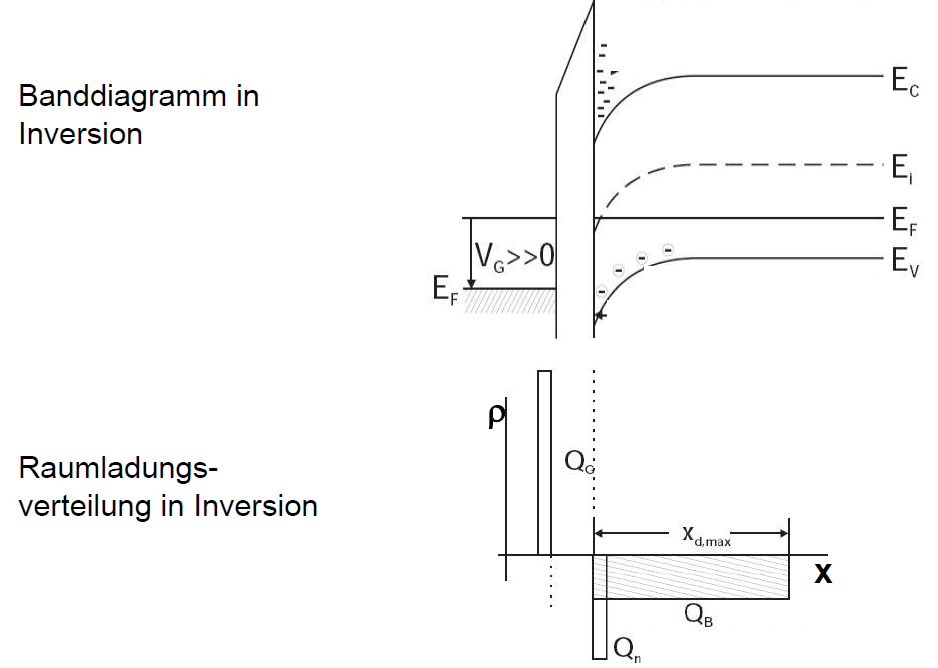
\includegraphics[width=0.60\linewidth]{Kapitel/Kap06/Inversion2}
		
		
\subsection{MOS-Transitoren}
MOS Transistoren sind Feldeffekttransistoren =
MOSFET
	\subsubsection{Grundaufbau}	
	Ein MOSFET ist ein aktives Bauelement mit mindestens drei Anschlüssen:
	\begin{itemize}
		\item S (source, dt. Quelle)
		\item D (drain, dt. Abfluss)
		\item G (gate, dt. Steuerelektrode)
		\item (B (bulk, dt. Substrat), Bei einigen Bauformen wird ein zusätzlicher Anschluss B nach außen geführt. Meistens ist das 		Substrat jedoch intern mit S verbunden )
	\end{itemize}
	Betrieb: Majoritätsladungsträger fließen von S nach D:
	\begin{itemize}
		\item unipolares Bauelement
		\item laterales Bauelement
	\end{itemize}
	Basierend auf dem Feldeffekt wird der Stromfluss wird durch ein an G anliegendes	elektrisches Feld gesteuert.
	\newline
	Die Geschwindigkeit ist vom Ladungsträgertransport von Source zum Drain abhängig. Dabei liegen die heutigen Kanallängen bei < 32 nm.
		%MOS Transistor
		\begin{center}
			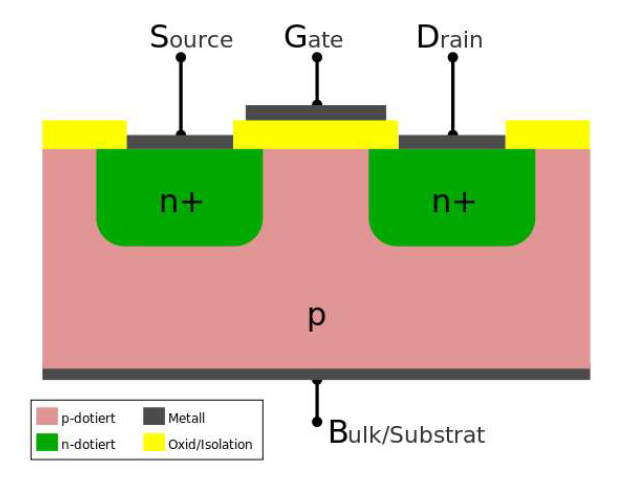
\includegraphics[width=0.7\linewidth]{Kapitel/Kap06/MOS_Transistor.png}
		\end{center}
	\subsubsection{neuere Entwicklungen}
		\textbf{Problem: }
		\newline
		Bei der Skalierung zu neuen Technologiegenerationen wird auch die Gateoxiddicke ebenfalls reduziert. 
		Die Tunnel/Leak-Ströme steigen exponentiell mit abnehmender Dicke.
		Irgendwann wäre man bei 3 Lagen von SiO2-Tetraedern. Die ist technisch nicht mehr homogen realisierbar (min. Schwankung 33 \%), da auch nicht mehr messbar. 
		\newline
		\textbf{Lösung: }
		\newline
		Daher muss trotz Skalierung das Dielektrikum dicker sein. Um die Kapazität bei größerer Dicke beizubehalten werden sogenannte High-K Dielektrika eingesetzt. 
		
		$C = \frac{\epsilon_r  \epsilon_0 A}{d}$ => Wird die Dicke d erhöht muss ein Material mit höherer Dielektrizitätskonstante $\epsilon_r$ (oder amerikanisch K) gefunden werden, um dieses auszugleichen.
	\subsubsection{Die vier Grundtypen}
	\subsubsection{Funktionsweise eines n-Kanal-Anreicherung-Transistoren}
	\subsubsection{Ausgangs- und Transferkennlinien}
\subsection{Anwendungen von MOS-Transistoren}
	
	\subsubsection{Vor- und Nachteile}
	\subsubsection{Funktionsprinzip eines CMOS-Inverter}


\todo{Fragen aus Own Clowd zuordnen}
\todo{Gruppenübungs-Inhalte ergänzen}
	
	% Kapitel 7
	\section{Kapitel 7 - Speicherbauelement }
	\todo{Wichtige Begriffe erklären}
\subsection{Flüchtige Speicher}
	\subsubsection{SRAM}
	Ladung in CMOS Inverter Flip-Flop
	6T-Zelle, sehr schnell
	
	\subsubsection{DRAM}
	Ladung in MOS-Kondensator
	1T-Zelle, wenig Platzbedarf, gute Skalierbarkeit
	Trench oder Stapel

\subsection{Nichtflüchtige Speicher}
	\subsubsection{ROM und PROM}
	\subsubsection{EPROM und EEPROM}
	Ladung auf floating gate
	elektrisch Schreiben und Löschen
	\subsubsection{Flash-EEPROM}
	\subsubsection{Solid State Devices}
	\subsubsection{Neuere Lösungen}
	Multibitspeicher
	Nanoclusterspeicher
	MRAM und FeRAM





\todo{Fragen aus Own Clowd zuordnen}
\todo{Gruppenübungs-Inhalte ergänzen}
	
	% Kapitel 8
	\section{Kapitel 8 - pn-Übergang }
	\todo{Wichtige Begriffe erklären}

\subsection{pn-Übergang}
	\subsubsection{Grundverhalten}
	 	Ein PN-(Homo-)Übergang liegt vor, wenn zwei Halbleiter aus dem selben Material in Kontakt sind, deren Dotierung unterschiedlich ist. 
	 	\newline
	 	Im thermischen Gleichgewicht ohne externes Feld  	bleibt das Ferminiveau konstant (Pinning)
	 	\newline
	 	\begin{center}
	 		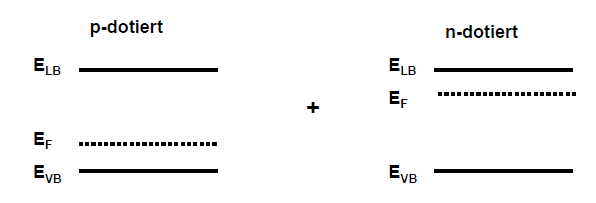
\includegraphics[width=0.6\linewidth]{Kapitel/Kap08/PN-uebergang_1.png}
		 	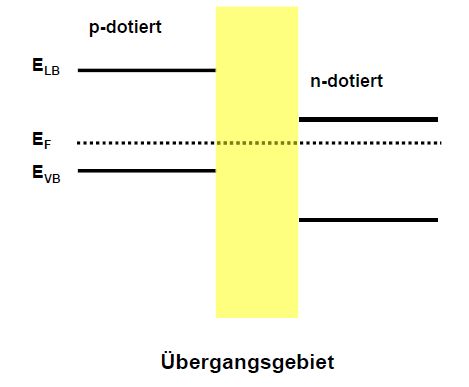
\includegraphics[width=0.35\linewidth]{Kapitel/Kap08/PN-uebergang_2.png}
		\end{center}
 	\subsubsection{metallurgische Grenze}
 		Der Punkt M, an dem die Dotierung sich von p zu n  	ändert, wird metallurgische Grenze genannt.
 		\begin{center}
 			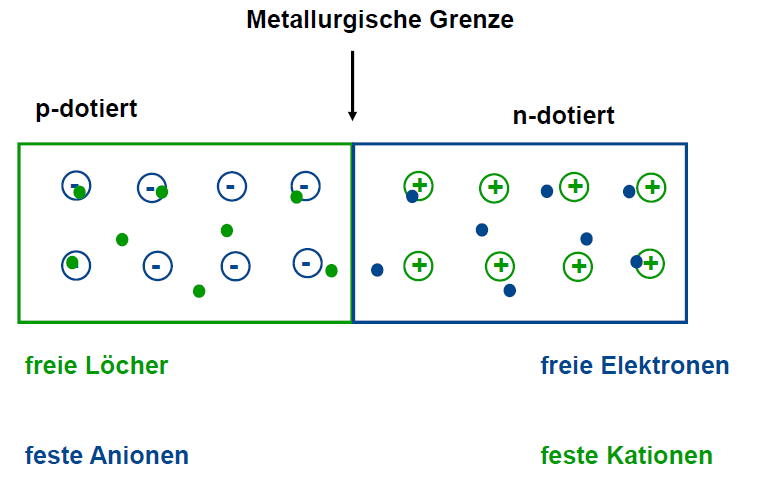
\includegraphics[width=0.4\linewidth]{Kapitel/Kap08/metallurgischeGrenze}
 		\end{center}
 		
 	\subsubsection{Diffusion und Drift}
 		\begin{enumerate}
 			\item Aufgrund des hohen Ladungsträgerkonzentrationsunterschiedes
 			kommt es zur Diffusion:
 			\begin{itemize}
 				\item von freien Löchern aus dem p-Gebiet ins n-Gebiet.
 				\item und von freien Elektronen aus dem n-Gebiet ins p-Gebiet
 			\end{itemize}
 			\item In der Nähe der Grenze M rekombinieren dann die diffundierten Ladungsträger mit den dortigen Majoritätsträgern.
 			\item Es kommt zu einer Verarmung der freien Ladungsträgern
 			\item Durch die verbleibenden festen Akzeptor-Ionen (p-Gebiet) und Donator-Ionen (n-Gebiet) entsteht ein lokales E-Feld entgegen der Diffusionsrichtung der Ladungsträger. Dies führt zu Driftströmen der freien Ladungsträgern.
 			\item Es stellt sich ein Gleichgewicht ein, so dass sich die Ladungsträgerströme resultierend aus Drift und Diffusion genau kompensieren.
 		\end{enumerate}
 		%drift und diffusion
		 \begin{center}
		 	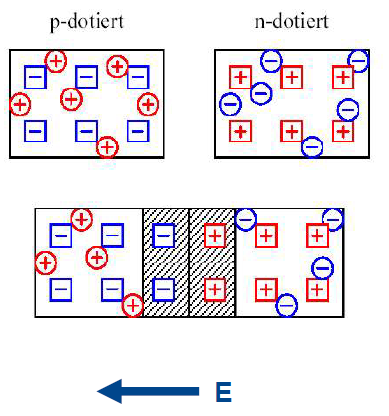
\includegraphics[width=0.4\linewidth]{Kapitel/Kap08/driftUndDiffusion}
		 \end{center}

	\subsubsection{Raumladungszone / Verarmungszone}
		Die Raumladungszone entsteht durch die Rekombination der freien Ladungsträger an der metallurigischen Grenze. Hierbei kommt es zur Verarmung der freien Ladungsträger, weshalb diese auch Veramungszone genannt wird. 
	\subsubsection{Eingebautes Feld}
	
		\begin{center}
			Zwischen den Festen Donator und Akzeptor-Ionen entsteht im Bereich der Raumladungszone ein elektrisches Feld.
			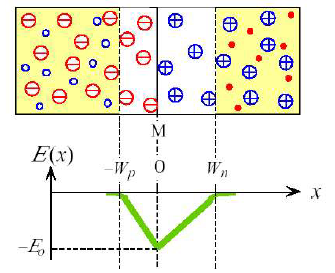
\includegraphics[width=0.4\linewidth]{Kapitel/Kap08/eingebautesFeld.png}
		\end{center}
		Den maximalen Wert $E_0$ des negativen elektrischen Feldes erreicht man an der Stelle der metallurgischen Grenze
		\newline
		Das elektrische Feld im thermischen Gleichgewicht wird eingebautes Feld genannt.
		
	\subsubsection{Diffusionsspannung}
		Die Spannung, die im thermischen Gleichgewicht über den pn-Übergang abfällt ($V_0$), wird auch 		eingebaute Spannung oder Diffusionsspannung ($U_D$) genannt.
		
		$V_0 = - \frac{E_0*W}{2}$
		
	\subsubsection{Breite der Raumladungszone}
		Die Breite der Raumladungszone hängt von den Donator- und Akzeptorkonzentrationen ab. Es gilt:			
		\begin{center}
			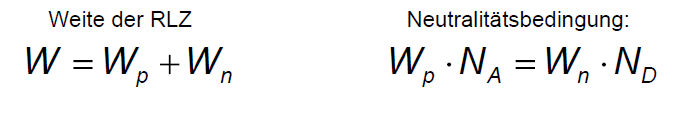
\includegraphics[width=0.5\linewidth]{Kapitel/Kap08/breiteRaumladungszoneNeutralisaetsbedingung.png}	
		\end{center}
	
		Daraus ergibt sich:	Für $N_A > N_D$ gilt $W_n > W_p$
		\newline
		Die Ausdehnung erfolgt immer stärker in das niedriger
		dotierte Gebiet.
		\newline
		Die Breite der Raumladungszone sinkt mit zunehmender Dotierung des n- bzw. p-Gebietes.
		\newline
		\textbf{Größenordnung Raumladungszone:}
		
		Annahme: Silizium mit p-Dotierung = n-Dotierung = $10^{18} cm^{-3}$
		
		Raumladungszone $W ca. 1 \mu m$
	
	\subsubsection{pn-Übergang mit externer Spannung}
	Externe Spannung V kann W vergrößern oder verkleinern:
	\begin{itemize}
		\item Für $V > V_0$ verschwindet die Raumladungszone -> Flussspannung 
		\item Für eine negative Spannung vergrößert sich die Raumladungszone -> Sperrspannung
	\end{itemize}
	\begin{center}
		\includegraphics[width=0.6\linewidth]{Kapitel/Kap08/pnUebergangExterneSpannung}
	\end{center}
	\begin{center}
		Gleichgewicht, Flussrichtung, Sperrrichtung
	\end{center}
	
\subsection{pn-Diode}
	Bei einer pn-Diode treffen ein p und ein n-Gebiet aufeinander. Durch Ablegung einer Spannung kann die Diode den Strom leiten, da die Raumladungszone gegen Null geht.
	\begin{center}
		\includegraphics[width=0.3\linewidth]{Kapitel/Kap08/Diode}
	\end{center}

	\subsubsection{Kennlinien für verschiedene Halbleitermaterialien}
		Größere Bandlücke verschiebt das Einsetzen des Stromes zu höheren Spannungen.
		\begin{center}
			\centering
			\includegraphics[width=0.7\linewidth]{Kapitel/Kap08/DiodeVerschiedeneHLMat.png}	
		\end{center}
	
	
	\subsubsection{Flusspolung, Sperrrichtung}
		\textbf{Flusspolung: }
		\begin{center}
			\includegraphics[width=0.5\linewidth]{Kapitel/Kap08/PNUebergangFlusspolung}
		\end{center}
		In Flussrichtung wird die Raumladungszone verringert und es kommt zu einem Stromfluss
		\newline
		\textbf{Sperrichtung:}
		\begin{center}
			\includegraphics[width=0.5\linewidth]{Kapitel/Kap08/sperrichtung}
		\end{center}
		In Sperrichtung ist kein großer Strom aufrecht zu
		erhalten. Es entsteht trotzdem ein kleiner Strom (Sperrstrom), da Minoritätsträger
		in die Raumladungszone diffundieren und dann
		durch das elektrische Feld ins gegenüberliegende
		Gebiet transportiert werden.
		Der Sperrstrom kann noch weitere Bestandteile haben, z. B. Oberflächenleckströme
		
	\subsubsection{Ideale Diodengleichung}
		\begin{center}
			Ideale Dioden-Gleichung oder Shockley-Gleichung.
			Wichtig hierbei ist, dass der Strom proportional exponentiell von der Bandlücke des Materials abhängt.
			\includegraphics[width=0.3\linewidth]{Kapitel/Kap08/IdealeDiodengleichung.png}
			\includegraphics[width=0.2\linewidth]{Kapitel/Kap08/IdealeDiodengleichungProportionalitaet.png}	
		\end{center}
	
	\subsubsection{Ideal vs. Real}
		\begin{center}
			\includegraphics[width=0.25\linewidth]{Kapitel/Kap08/IdealvsReal.png}
			\includegraphics[width=0.35\linewidth]{Kapitel/Kap08/RealeDiode}
			
		\end{center}

	\subsubsection{Idealitätsfaktor}
		In realen pn-Übergängen tritt eine gewisse Rekombination in der Raumladungszone auf, was zu einem zusätzlichen äußeren Strom führt. 
		Gesamtstrom in einer pn-Diode ergibt sich daher aus der Summe des idealen Diodenstromes mit dem
		Rekombinationsstrom in der RLZ:
		\newline
		Bei der Beschreibung von realen Diodencharakteristiken in bestimmten Spannungsbereichen wird dabei folgende Gleichung verwendet (Gleichung irrelevant)
		\begin{center}
			\includegraphics[width=0.3\linewidth]{Kapitel/Kap08/genaherteGleichung}
		\end{center}
		Der darin enthaltene \textbf{ Faktor $\eta$ wird als Idealitätsfaktor bezeichnet und liegt immer zwischen 1 und 2}
		\begin{center}
			\includegraphics[width=0.5\linewidth]{Kapitel/Kap08/IdealitaetsfaktorBeispiel}
		\end{center}
		
	\subsubsection{Temperaturabhängigkeiten}
		Bei wachsender Temperatur nimmt der ideale
		Stromanteil gegenüber dem nichtidealen zu. Die Einsatzspannung der Diode sinkt.
		\begin{center}
			\includegraphics[width=0.25\linewidth]{Kapitel/Kap08/temperaturabhaengigkeit1}
		\end{center}
		Mit wachsender Temperatur nimmt auch der Sperrstrom zu
		\begin{center}
			\includegraphics[width=0.25\linewidth]{Kapitel/Kap08/temperaturabhaengigkeit2}
		\end{center}
		
	
	\subsubsection{Durchbruch}
	Die pn-Diode kann nicht mit beliebig großer Spannung in Sperrichtung betrieben werden.
	Eine zu hohe Spannung in Sperrichtung führt dazu, dass die Diode "durchbricht". Der Strom steigt ab einer kritischen Sperrspannung (Durchbruchsspanung) sehr stark an. 
	\subsubsection{Lawinendurchbruch}
	Durch ausreichend hohe Sperrspannungen ist es 	möglich, die Raumladungszone und damit das 	elektrische Feld am pn- Übergang soweit zu vergrößern, 	dass die beschleunigten Ladungsträger ausreichend hohe Energien erreichen, um ihrerseits durch Stöße mit Kristallatomen weitere Elektron-Loch-Paare zu erzeugen (Stoßionisation).
	Die so generierten Elektronen und Löcher können bei ausreichender Beschleunigung im elektrischen Feld ihrerseits wieder Stoßionisationprozesse auszulösen.
	Somit kommt es zu einer Lawinenartigen Bildung von Ladungsträgern, der Sogenannte Lawinendurchbruch.
	\subsubsection{Zener-Effekt/-Diode}
	Der Zener-Effekt tritt bei hoch
	dotierten pn-Übergängen auf, in denen schmale Raumladungszonen und hohe elektrische Feldstärken auftreten.
	In diesem Fall kann es unter Sperrspannung zum Tunneln von Elektronen des Valenzbandes der p-Seite ins Leitungsband der n-Seite kommen, wobei auch Elektron-Lochpaare in der RLZ geschaffen werden. Dies führt zu einem Starken Anstieg des Stroms. Die kritische Spannung liegt dabei niedriger als die Durchbruchsspannung. 
	\newline
	Die auf diesem Effekt basierende Z-Dioden erlaubt es, dass sie in zahlreichen Schaltungen zur Stabilisierung und
	Begrenzung von elektrischen Spannungen eingesetzt werden.
	\begin{center}
		\includegraphics[width=0.3\linewidth]{Kapitel/Kap08/Zenerdiode}
	\end{center}
	
	\subsubsection{Varaktordioden}
		In Sperrrichtung wirkt die Sperrschicht bzw. Raumladungszone am pn-Übergang wie eine Kapazität.
		Ändert sich die Spannung an der Diode ändert sich auch die Kapazität der Sperrschicht.
		Die Varaktordiode wird daher als spannungsabhängige Kapazität (Varaktor) genutzt.
		Hierbei ist die Sperrschicht-Kapazität
		besonders groß. Dadurch sind große Kapazitätsänderungen möglich.
		\begin{center}
			\includegraphics[width=0.3\linewidth]{Kapitel/Kap08/Varaktordiode}
		\end{center}
		
	
	\subsubsection{Diodentypen und ihre Anwendungsfelder}
		Vermutlich eher unwichtig:
		\begin{itemize}
			\item Optik -> Laserdiode, Fotodiode, LED
			\item Kapazitive Dioden
			\item Gesteuerte Gleichrichter und verwandte Bauelemente -> Vierschichtdioden, Thyristor
			\item diverse weitere
		\end{itemize}


\todo{Fragen aus Own Clowd zuordnen}
\todo{Gruppenübungs-Inhalte ergänzen}
	
	% Kapitel 9
	\section{Kapitel 9 - Solarzelle }
	

\todo{Wichtige Begriffe erklären}


\subsection{Nutzung von Sonnenenergie}

	\subsubsection{Gegenwärtige Energiequellen}

	\subsubsection{Mögliche Entwicklungen}


\subsection{Funktionsweise einer Solarzelle}

	\subsubsection{Grundprinzip}

	\subsubsection{Warum braucht man eine pn-Struktur}

	\subsubsection{Wirkungsgrade, Ursachen für Verluste}

\subsection{Typen von Solarzellen}

	\subsubsection{Verschiedene Materialien}

	\subsubsection{Verschiedene Konstruktionen}




\subsection{Auslaufen der Energie Reserven}

Kohle ca. 100 Jahre

Erdgas und Erdöl ca. 50 Jahre

Uran ca. 70 Jahre


\subsection{Anteile an Erneuerbaren Energie}

Vor allem Skandinavien

Deutschland 38,5\% am gesamten Strommix


\subsection{Massendefekt}

Masse $\leftrightarrow$ Energie: $E = m\cdot c^2$

Massendefekt = Bindungsenergie

Diese Energie wird bei Kernumwandlungen freigesetzt


\subsection{Kernfusion}

$Deuterium H^3 + Tritium H^2 \rightarrow Heliumkern He^2 + n$


\subsection{Geschichte}

Erste Solarzelle (1954)

4-6\% Wirkungsgrad


\subsection{Vorteile Solarenergie}

Unbegrenzt vorhanden

Emissionslos

Reduzierung von energiepolitischen Abhängigkeiten


\subsection{Nachteile Solarenergie}

Nicht konstant (Wetter, Jahreszeiten, Tageszeiten...)

Herstellung nicht emissionsfrei

Hohe Kosten


\subsection{Brandenburg ist toll}


\subsection{Aufbau}

95% aler Solarzellen aus Silizium

np-Halbleiter Aufbau

n Schicht ist sehr dünn, damit das Licht an den pn-Übergang gelangen kann


\subsection{Photoelektrischer Effekt}

Äußerer (nicht für Solarzellen relevant)

Aufgeladene Oberfläche gibt Elektronen bei Bestrahlung ab

Innerer (relevant für Solarzellen)

besser Leitfähigkeit bei Beleuchtung, da Elektronen auf höheres Valenzband gehoben werden


\subsection{Ablauf}

Licht sorgt dafür, dass Elektronen in die n Schicht und Löcher in die p Schicht wandern. Können an Kontakten abgegriffen werden.

Elektronen-Loch-Paare müssen vor der Rekombination getrennt werden

Spannung immer ähnlich (0.5 V bei Silizium), Strom steigt mit Beleuchtungsstärke an

Leistung ist temperaturabhängig


$Stromabgabe = Generation - Rekombination = J = J_SC - J_0 \bigg(e^{\frac{qV}{kT}}-1\bigg)$

Rekombination = Dunkel-Diodenstrom

Keine Annahme über pn- Übergang für die Formale notwendig


Der pn-Übergang ist für die Kontaktierung. Die Fermi.Level der Metallkontakte richtet sich nach dem der angrenzenden Majoritäten

Somit könne die Löcher durch p und Elektronen durch n Halbleiter kontaktiert werden. Fließen nach außen ab.


Kennlinie wie bei einer Diode, aber verschiebt sich bei Sonneneinstrahlung


Maximum Power Point bei P=J*V = max

Füllfaktor ist Verhältnis zwischen Leistung und MPP


\subsection{Wirkungsgrad}

MPP / Lichtintensität

Photonen nicht energetisch genug ($hv < E_g$)

Photonen haben Überschussenergie die in Wärme umgesetzt wird ($hv > E_g$)

Abschattung durch Kontakte

Widerstandsverluste

Es kann nicht das gesamte Spektrum genutzt werden

Theoretisch auf 32,2\% bei Licht von 1,12 ev begrenzt


\subsection{Verschiede Arten}

Monokristalines Silizium 16-22\%

am besten, aber auch teuer

Polykristalines Silizium 15-16\%

verbreiteter, da billiger

Amporphes Silizium 	6-8\%


\subsection{Neue Wege}

\begin{itemize}

	\item Anschlüsse von hinten

	\item Oberflächentexturierung zur Flächen Maximierung z.B. auf-ätzen

	\item Bündeln mit z.B. Linsen

	\item Mehrere Zellen für verschiedene Wellenlängen hintereinander

\end{itemize}s



\todo{Fragen aus Own Clowd zuordnen}

\todo{Gruppenübungs-Inhalte ergänzen}



	
	% Kapitel 10
	\section{Kapitel 10 - Bipolartransistor }
	\subsection{Bipolartransistor versus Feldeffekttransistor}
	\subsubsection{Einfluss der Skalierung}
	\paragraph{Feldeffekttransistor FET}
	Ladungsträgertransport erfolgt von Source
	nach Drain. Ein FET ist ein laterales Bauelement und ist somit durch die Lithografie eingeschränkt (Kanallängen < 22nm).
	
	\todo{Ist das bei der MOS Vorlesung schon drin?}
	\paragraph{Bipolar Transistor HBT}
	Ladungsträgertransport erfolgt vom Emitter
	zum Kollektor. Ein HBT ist ein vertikales Bauelement und ist somit durch die Schichtdicke eingeschränkt (Basisdicke < 25 nm). Mehr oder weniger unabhängig von den lateralen Abmessungen.
	\subsubsection{Grundeigenschaften}
	\subsubsection{Anwendungsfelder}
	
\subsection{Bipolartransistor (Homojunktion, BJT)}
	\subsubsection{npn versus pnp}
	Der unterschied von npn und pnp Transitoren liegt im Aufbau. Die Bezeichnungen stehen dabei im direkten Zusammenhang mit der Abfolge der Schichten. So besteht der ein npn-Transistor aus zwei n-dotierten Schichten mit einer Basis aus p-dotierten Material. Der pnp-Transistor genau umgekehrt. Bei dem Schaltsymbol handelt es sich in beiden fällen um einen Strich, der von links mit der Basis (B) und von rechts mit 2 Schrägen, dem Kollektor (C) und dem Emitter (E) verbunden sind (\ref{10_npn_pnp}).  
	\begin{figure}[h]
		\centering
		\includegraphics[width=0.4\textwidth]{Kapitel/Kap10/npn_pnp.png}
		\caption{npn- und pnp-Transistor im Vergleich}
		\label{10_npn_pnp}
	\end{figure}

	\subsubsection{Kenngrößen}
	\begin{figure}[h]
		\centering
		\includegraphics[width=0.4\textwidth]{Kapitel/Kap10/groessen.png}
		\caption{Unterschiedliche Kenngrößen am Bipolartransistor}
		\label{10_groessen}
	\end{figure}
	Es gibt 4 unterschiedliche Kennlinienfelder (\ref{10_kennlinie}), die einen Transistor charakterisieren.
	\paragraph{Eingangskennlinienfeld} Es wird der Basisstrom $I_B$ gegen die Basisspannung $U_{BE}$ aufgetragen. Da der Basis-Emitter Übergang als Diode gesehen werden kann, sieht diese Kennlinie wie eine Diode aus.
	\paragraph{Ausgangskennlinienfeld} Das Ausgangskennlinienfeld stellt den Kollektorstrom $I_C$ in Abhängigkeit von der Kollektor-Emitter-Spannung $U_{CE}$ und dem Basisstrom $I_B$ dar.
	\paragraph{Übertragungskennlinienfeld} Hierbei wird der Kollektorstrom $I_C$ gegen einen Basisstrom $I_B$ bei einer festgelegten Kollektor-Emitter-Spannung $U_{CE}$ aufgetragen.
	\paragraph{Spannungsrückwirkungskennlinienfeld} Dieses beschreibt die Rückwirkung der Kollektor-Emitter-Spannung $U_{CE}$ auf die Basisspannung $U_BE$ bei unterschiedlichen Basisströmen $I_B$
	\begin{figure}[h]
		\centering
		\includegraphics[width=0.6\textwidth]{Kapitel/Kap10/kennlinien.png}
		\caption{Kennlinienfelder eines Bipolartransistors}
		\label{10_kennlinie}
	\end{figure}
	  
	\subsubsection{Funktionsprinzip}
	Die drei Schichten wirken wie eine Diode. Zur Funktion muss der von Kollektor nach Emitter ein positive Spannung abfallen. Durch ein Potential an der Basis kann dann der Stromfluss auf dieser Strecke gesteuert werden.
	Im Ruhezustand bilden sich jeweils an den beiden Grenzflächen Sperrschichten aus (\ref{10_zustände} - 1). Wir nun eine positive Kollektor-Emitter-Spannung angelegt, verändern sich diese. Dabei wird die Sperrschicht zwischen Kollektor und Basis größer und zwischen Basis und Emitter kleiner (\ref{10_zustände} - 2). In diesem Zustand ist noch kein Stromfluss von Kollektor nach Emitter möglich. Wird nun noch eine gegenüber dem Emitter positive Spannung an die Basis angelegt, so kommt es zum Stromfluss (\ref{10_zustände} -3 ). Dabei ist in den Grafiken zu beachten, dass es sich bei den Spannungs- und Strom angaben um die technische, nicht die physikalische Stromrichtung handelt. Aus diesem Grund fließen die Elektronen vom Emitter zum Kollektor, obwohl die Spannung in die andere Richtung anliegt. Im letzten Zustand ist die Sperrschicht zwischen Basis und Emitter nun komplett abgebaut. Dies geschieht durch die Rekombination der Ladungen in der Basis. Diese muss sehr dünn sein, damit es nicht zu zu vielen Rekombinationen kommt. Die meisten Elektronen fließen weiter zum Kollektor (etwas 99\%).
	\begin{figure}[h]
		\centering
		\includegraphics[width=0.4\textwidth]{Kapitel/Kap10/zustand_1.png}
		\includegraphics[width=0.4\textwidth]{Kapitel/Kap10/zustand_2.png}
		\includegraphics[width=0.4\textwidth]{Kapitel/Kap10/zustand_3.png}
		\caption{Unterschiedliche Zustande eines npn-Transistors}
		\label{10_zustände}
	\end{figure}
	Man kann nun den Kollektor und Basisstrom messen. Der Quotient beider ergibt die Stromverstärkung.
	\begin{align}
		\beta = \frac{I_C}{I_B}
		\label{10_beta}
	\end{align}
	Ein pnp-Transistor funktioniert nach dem selben Prinzip, nur sind alle Polaritäten der Strom und Spannungen umgekehrt.
	
	\paragraph{Early Effekt} Der Early-Effekt(Basisweiten-Modulation) beschreibt die Abhängigkeit des Stroms von der Kollektor-Emitter-Spannung. Wird die Spannung erhöht, so wird die Raumladungszone des Kollektor-Basis-Übergangs größer. Dementsprechend nimmt die Weite der Basis ab. Dies hat zur folge, dass man aus Transistoren keine idealen Stromquellen bauen kann. Je größer die Early-Spannung ist desto konstanter ist der Strom des Transistors.
	
	\subsubsection{Betriebsarten}
	Ein Bipolartransistor kann sich in 4 unterschiedlichen Betriebsarten befinden (\ref{10_betriebsarten}).
	\begin{table}[h]
		\centering
		\begin{tabular}{c|c|c}
			Betriebsart& EB-Übergang &CB-Übergang\\
			\hline
			Sättigung & Fluss & Fluss\\
			Aktiv (Normal) & Fluss & Sperr\\
			Invertiert & Sperr & Fluss\\
			Sperrbetrieb & Sperr & Sperr
		\end{tabular}
		\caption{Unterschiedliche Betriebsarten des Bipolartransistors}
		\label{10_betriebsarten}
	\end{table}
	\paragraph{Sperrbereich} Beide Übergänge sperren. Theoretisch stell dies einen offenen Schalter dar, dementsprechend sollte kein Strom fließen, allerdings gibt es geringe Leckströme. Der Transistor ist somit kein idealer Schalter.
	\paragraph{Aktiv} Dieser Bereich wird auch Normalbetrieb oder Verstärkerbereich genannt. Die Emitterdiode ist in Flussrichtung und die Kollektordiode in Sperrrichtung. Näherungsweise gilt die Formel für die Stromverstärkung (\ref{10_beta}). Der Transistor wird üblicherweise nur so betrieben, das diese Verstärkung über die Stromänderung annähernd konstant bleibt. 
	\paragraph{Sättigung} In diesem Bereich leiten beide Dioden. Die Basis enthält allerdings mehr Ladungsträger als notwendig, welche beim ausschalten zunächst abtransportiert werden müssen. In diesem Bereich verhält sich der Transistor wie ein Schalter mit konstanten Durchgangswiderstand.
	\paragraph{Invertiert} In diesem, auch inverser Verstärkerbereich, genannten Zustand ist der Basis-Kollektor-Übergang in Durchlassrichtung und der Basis-Emitter-Übergang in Sperrrichtung. Alles funktioniert hier wie im normalen Verstärkerbereich, allerdings ist die Stromverstärkung wesentlich geringer. 
	\subsubsection{Grundschaltungen}
\subsection{Heterojunktion Bipolartransistor (HBT)}
	\subsubsection{Aufbau}
	\subsubsection{Vorteile gegenüber BJT}
	\subsubsection{Erreichbare Leistungen}
	\subsubsection{Modulare Integration}


\todo{Fragen aus Own Clowd zuordnen}
\todo{Gruppenübungs-Inhalte ergänzen}
	
	% Kapitel 11
	\section{Kapitel 11 - Verbindungshalbleiter }
	\todo{Wichtige Begriffe erklären}
\subsection{Element- und Verbindungshalbleiter}
	\subsubsection{Direkte und indirekte Halbleiter}
	Direkte und indirekte Halbleiter unterscheiden sich in der Position des Minimums / Maximums im Bänderdiagramm .......
	
		\includegraphics[width=\linewidth]{Kapitel/Kap11/direkte_indirekte_halbleiter.PNG}
	
	\subsubsection{Dotieren von Verbindungshalbleitern}	
	\subsubsection{Ladungsträgerbeweglichkeiten}
\subsection{Welleneigenschaften}
	\subsubsection{Monochromatisch} 
	\subsubsection{kohärent} \subsubsection{kollimiert}
\subsection{Leuchtdioden}
	\subsubsection{Funktionsprinzip}
	\subsubsection{Verschiedene Farben}
	\subsubsection{Weiße Dioden}
\subsection{Laser}
	\subsubsection{Funktionsprinzip (stimulierte Emission, Pumpen, beteiligte Energieniveaus, ...)}
	
	\subsubsection{Resonatoren}
	\subsubsection{Halbleiterlaser (Prinzipeller Aufbau, VCSEL, ...)}


\todo{Fragen aus Own Clowd zuordnen}
\todo{Gruppenübungs-Inhalte ergänzen}
	
	% Kapitel 12
	\section{Kapitel 12 - Technologie }
	\todo{Wichtige Begriffe erklären}


\subsection{Technologieverfahren}
	\subsubsection{}
	\subsubsection{}
	\subsubsection{}
\subsection{}
	\subsubsection{}
	\subsubsection{}
	\subsubsection{}
\subsection{}
	\subsubsection{}
	\subsubsection{}
	\subsubsection{}
\subsection{}
	\subsubsection{}
	\subsubsection{}
	\subsubsection{}
\subsection{}
	\subsubsection{}
	\subsubsection{}
	\subsubsection{}

\todo{Fragen aus Own Clowd zuordnen}
\todo{Gruppenübungs-Inhalte ergänzen}
	
	% Kapitel 13
	\section{Kapitel 13 - Nanoelektronik }
	\subsection{Begrifflichkeit}
	Man unterscheidet die Begriffe Mirko- und Nanoelektronik. Sobald die Strukturen kleiner als 100nm groß sind befindet man sich im Bereich der Nanoelektronik. Jedoch kann man nicht immer einfach alles kleiner skalieren. aus diesem Grund müssen neue Technologien und Materialien verwendet werden.
\subsection{Showstopper für aquivaltes Skalieren}
	\begin{itemize}
		\item Physikalische Grenzen (z.B. Quanteneffekte)
		\item Grenzen der konventionellen Bauelementkonzepte
		\item Leistung und Wärme
		\item Grenzen der verwendeten Materialien
		\item Technische Gründe (z.B. Lithografie)
		\item Ökonomische Grenzen
		\item Grenzen beim Entwurf
	\end{itemize}
\subsection{FET}
	Für die Skalierung von Transistoren ist es notwendig, High-K Materialien als Isolator zu verwenden, damit der MOS Kondensator trotz dem geringen Größe immer noch einen ähnlichen Effekt aufweist. Außerdem gibt es ein Konzept, bei dem der Transistor nicht in die Tiefe aufgebaut ist, sondern auf der Fläche verteilt(KrisMOS). Man kann das Gate auch um einen Kanal herum aufbauen. Somit hat man eine große Einwirkung auf diesen.
\subsection{RC-Verzögerung}
	Nehmen wir an, wir haben 2 parallele Leiter. Soll sich ein Signal auf diesen verändern so kommt es durch kapazitive Effekte zu RC Verzögerungen. Jedoch sind viele Parameter durch das Design beschränkt, so lässt sich z.B. der Anstand zwischen den Leitungen nur schwer ändern. Aus diesem Grund ist es notwendig, Metallleitungen zu verwenden, welche einen sehr geringen Widerstand besitzen oder das Material zwischen den Leitern zu verändern.
\subsection{Zukünftige Elektronik}
	Es gitb mehrere Ideen, mit welchen die zukünftige Elektrik verbessert werden kann.
	\begin{itemize}
		\item Keine planaren, sonder dreidimensionale Chips
		\item Molekulare oder Kohlenstoffbasierte Elektronik
		\item Nanodräht
		\item Optische Kommunikation
	\end{itemize}

	
	
	% Beispiele 
	% Kapitel 0
	\section{Test}
	% in-line formeln
abdcdasd $\sum_{n=1}^{k}\rho_n$
% formeln als Block
\begin{align*} 
	\sum_{n=1}^{k}\rho_n
\end{align*}

%sehen unterschiedlich aus

\subsection{Thema 1}
	absasfasdf
\subsection{Thema 2}
	
	\begin{itemize}
		\item Halbleiter1
		\begin{enumerate}
			\item Montag
			\item Montag
			\item Montag
			\item Montag
		\end{enumerate}
		\item Halbleiter2
	\end{itemize}
	\includegraphics[width=\linewidth]{Kapitel/Kap01/test.png}
	\begin{center}
		
	
		\includegraphics[width=0.4\linewidth]{Kapitel/Kap01/test.png}
	\end{center}


\begin{tabular}{|l|r|}
	\hline
	\textbf{Hello} & World\\
	\hline
	Hello & Martin\\
	\hline
\end{tabular}
\todo{Hello WOlrd}

\subsection{Verteilungsfunktion}
\subsubsection{Fermiverteilung}


Definition der Fermi-Energie
Lage des Fermi-Niveaus (intrinsisch vs. dotiert)
Effektive Zustandsdichten
Ladungsträger im Halbleiter
Massenwirkungsgesetz
Neutralitätsbedingung
Intrinsische Ladungsträgerkonzentration
Bezeichnung von dotierten Halbleitern
Majoritäten und Minoritäten
Ladungsträgerbewegung
Driftstrom, Sättigung usw.
Diffusionsstrom
Temperaturspannung
Leitfähigkeit von Halbleitern
p- und n-Typ, Temperaturabhängigkeit usw.
Definitionen von Dotierniveaus


% geometry package --> Seitenränder einstellen
	
	
	
	
	
	% Aufgabe 2
	%\section{}
	%\input{./Kapitel/Aufgabe2}
	
	% Aufgabe 3
	%\section{}
	%\input{./Kapitel/Aufgabe3}
	
\end{document}